\documentclass[a4paper,twoside,openright,11pt]{book}

\usepackage{setspace}
\usepackage{layout}
\usepackage{geometry}
\geometry{bindingoffset=1cm}

\usepackage{amsmath}
\usepackage{amssymb}
\usepackage{tensor}
\usepackage{array}
\usepackage{amsthm}
\usepackage{amsfonts}
\usepackage{amstext}
\usepackage{mathtools}
\usepackage{makeidx}
\usepackage[pdftex]{graphicx}
\usepackage{epstopdf}
\usepackage{url}
\usepackage{epigraph}
\usepackage{hyperref}
\usepackage{enumitem}

\usepackage{fancyhdr}

\usepackage{hyperref}

\usepackage{type1cm}
\usepackage{lettrine}

\usepackage{color}
\usepackage{colortbl}
\usepackage{placeins}

\usepackage{multirow}
\usepackage[small]{caption}
\usepackage{subcaption}

\usepackage{titlesec}
\titleformat{\chapter}[display]
{\normalfont\bfseries\filcenter}
{\LARGE\thechapter}
{1ex}
{\titlerule[2pt]
\vspace{2ex}%
\LARGE}
[\vspace{1ex}%
{\titlerule[2pt]}]

\usepackage{appendix}

\usepackage{algorithmic, algorithm}

\usepackage[squaren, Gray, cdot]{SIunits}

\usepackage{rotating}

\usepackage{tikz, pgfplots}
\usepackage{tikz-qtree}
\usetikzlibrary{patterns}

\usepackage{import}

\renewcommand{\algorithmicrequire}{\textbf{Input:}}
\renewcommand{\algorithmicensure}{\textbf{Output:}}

% Setup pdf meta-data.
\hypersetup{ % Modifiez la valeur des champs suivants
pdfauthor = {Antonio El Khoury},
pdftitle = {Planning Optimal Motions for Anthropomorphic Systems},
pdfsubject = {Planning Optimal Motions for Anthropomorphic Systems},
pdfkeywords = {Motion Planning, Optimal Control, Humanoid Robot},
pdfcreator = {Antonio El Khoury},
pdfproducer = {Antonio El Khoury}
}

% Customize chapter head.
\makeatletter
\renewcommand\chapter{\if@openright\cleardoublepage\else\clearpage\fi
                    %\thispagestyle{empty}%
                    \global\@topnum\z@
                    \@afterindentfalse
                    \secdef\@chapter\@schapter}
\def\@makechapterhead#1{%
  \vspace*{50\p@}%
  {\parindent \z@ \raggedright \normalfont
    \ifnum \c@secnumdepth >\m@ne
      \if@mainmatter
        \Huge\bfseries\@chapapp~\thechapter\\\vskip 20\p@
      \fi
    \fi
    \Huge \bfseries #1\par\nobreak
    \vskip 40\p@
  }}
\makeatother

% Enforce math style.
\everymath{\displaystyle}

% Generate index.
\makeindex

% Please fancyhdr.
\pagestyle{headings}
\setlength{\headheight}{26pt}
\setlength{\footskip}{120pt}

% Align bibliography left and add some padding
\makeatletter
\renewcommand{\@biblabel}[1]{[#1]\hfill\hspace{0.25cm}}
\makeatother

% Custom commands.
\newcommand{\transformation}[2]{%
\ensuremath{{}^{#1}\!\text{M}_{#2}}}

\newcommand{\HRule}{\rule{\linewidth}{0.5mm}}

\newcolumntype{L}[1]{>{\raggedright\let\newline\\\arraybackslash\hspace{0pt}}m{#1}}
\newcolumntype{C}[1]{>{\centering\let\newline\\\arraybackslash\hspace{0pt}}m{#1}}
\newcolumntype{R}[1]{>{\raggedleft\let\newline\\\arraybackslash\hspace{0pt}}m{#1}}

\newcommand{\config}[1]{$\mathbf{q_{#1}}$}
\newcommand{\espace}{$\mathbb R^n$}
\newcommand{\task}[1]{$\mathbf{x_{#1}}$}
\newcommand{\tspace}[1]{$\mathbb R^{#1}$}
\newcommand{\wspace}{$\mathcal{WS}$}
\newcommand{\cspace}{$\mathcal{CS}$}
\newcommand{\cfree}{$\mathcal{CS}_{free}$}
\newcommand{\cobs}{$\mathcal{CS}_{obs}$}
\newcommand{\ctree}{$\mathcal{T}$}
\newcommand{\segroup}{$SE(3)$}
\newcommand{\actcspace}{$\mathcal{Q}$}
\newcommand{\robot}{$R$}
\newcommand{\body}[1]{$B_{#1}$}
\newcommand{\joint}[1]{$J_{#1}$}

\newtheorem{theorem}{Theorem}
\renewcommand{\labelitemi}{$-$}
\newcommand{\manifold}{\mathcal{M}}
\newcommand{\goalmanifold}{\mathcal{M}_{g}}

\newcommand{\state}[1]{$\mathbf{x_{#1}}$}
\newcommand{\sspace}{$\mathcal{SS}$}
\newcommand{\dotstate}[1]{$\mathbf{\dot{x}_{#1}}$}
\newcommand{\control}[1]{$\mathbf{u_{#1}}$}
\newcommand{\dfcn}[1]{$\mathbf{f_{#1}}$}
\newcommand{\eqcstr}[1]{$\mathbf{g_{#1}}$}
\newcommand{\ineqcstr}[1]{$\mathbf{h_{#1}}$}
\newcommand{\bndcstr}[1]{$\mathbf{r_{#1}}$}
\newcommand{\dotconfig}[1]{$\mathbf{\dot{q}_{#1}}$}
\newcommand{\ddotconfig}[1]{$\mathbf{\ddot{q}_{#1}}$}
\newcommand{\dddotconfig}[1]{$\mathbf{\dddot{q}_{#1}}$}

\newcommand{\argmin}[1]{\mathbf{#1}^{\star}}
\newcommand{\arginit}[1]{\mathbf{#1}_0}
\newcommand*\circled[1]{\tikz[baseline=(char.base)]{
            \node[shape=circle,draw,inner sep=1pt] (char) {#1};}}
\newcommand{\norm}[1]{\left\lVert #1 \right\rVert}
\newcommand{\overbar}[1]{\overline{#1}}
\newcommand{\downbar}[1]{\underline{#1}}

%%%%%%%%%%%%%%%%%%%%%%%%%%%%%%%%% DOCUMENT %%%%%%%%%%%%%%%%%%%%%%%%%%%%%%%%%%%%%

\begin{document}
\bibliographystyle{these}
%
%\layout
%\doublespacing
%\onehalfspacing
%
\author{Antonio El Khoury}
\title{Awesome Title}
\date{Juin 2013}
%
%% \thispagestyle{empty}
%% \begin{tikzpicture}[remember picture, overlay]
%%  \node[inner sep=0pt] at (current page.center) {
%%   \includegraphics[width=\paperwidth,height=\paperheight]{couverture}
%% };
%% \end{tikzpicture}
%
%\frontmatter
\tableofcontents{\thispagestyle{headings}}
%
%\mainmatter
%\pagestyle{empty}
%\chapter*{Remerciements}

J'ai profit\'e d'un accueil exceptionnel au LAAS-CNRS durant mes trois
ann\'ees de th\`ese. C'est pourquoi je tiens tout d'abord \`a
remercier ses directeurs successifs Raja Chatila, Jean-Louis Sanchez
et Jean Arlat, le directeur du th\`eme Robotique Rachid Alami, et plus
sp\'ecifiquement les directeurs successifs du groupe Gepetto Jean-Paul
Laumond et Philippe Sou\`eres.

Je tiens \`a exprimer toute ma gratitude envers mes directeurs de
th\`ese Florent Lamiraux et Michel Ta\"ix. Leur confiance, leurs
connaissances approfondies, leurs pr\'ecieux conseils et leur
sympathie ont directement contribu\'e au travaux que j'ai effectu\'es
et au plaisir que j'en ai tir\'e.

C'est un honneur d'avoir Maren Bennewitz et Abderrahmane Kheddar comme
rapporteurs de ma th\`ese, et je les remercie sinc\`erement pour leur
relecture attentive de mon manuscrit. Je remercie \'egalement Brigitte
d'Andr\'ea-Novel, Timothy Bretl, Patrick Dan\`es et Rodolphe Gelin
d'avoir accept\'e de faire partie de mon jury de th\`ese, ainsi que
pour leurs remarques et discussions int\'eressantes.

J'ai eu la chance d'effectuer un s\'ejour scientifique \`a
l'Universit\'e de Heidelberg dans le groupe ORB . Je tiens \`a
remercier Katja Mombaur pour ses pr\'ecieux conseils et l'excellent
accueil qu'elle m'a r\'eserv\'ee.

J'ai \'et\'e tr\`es marqu\'e par l'esprit d'\'equipe qui r\`egne dans
le groupe Gepetto, et esp\`ere y avoir contribu\'e durant ces trois
ann\'ees. Je remercie chaleureusement Nicolas Mansard et Olivier
Stasse qui, sans \^etre directement impliqu\'es dans mes travaux,
m'ont fourni tout le soutien scientifique et technique dont un
doctorant pourrait r\^ever.

\bigskip

Ces trois derni\`eres ann\'ees sont pass\'ees rapidement; ceci est
principalement d\^u \`a mon c\^otoiement au quotidien de doctorants et
stagiaires sympathiques et brillants, dont la bonne humeur a ajout\'e
encore plus de plaisir \`a ces travaux de recherche. J'ai eu la joie
de collaborer \'etroitement avec S\'ebastien Dalibard, Martin Felis,
David Flavign\'e et Thomas Moulard; je les remercie pour leur
d\'evouement \`a nos travaux ainsi que pour leur amiti\'e.

Je me sens privil\'egi\'e d'avoir pu rencontrer de glorieux anciens,
qui m'ont inculqu\'e les pr\'eceptes de l'esprit d'\'equipe et de la
bonne ambiance. Merci donc \`a Duong, Fran\c{c}ois, Layale, Manish,
Maxime, Nicolas, Oussama, Samory, Sovan, Valentin, Wassim, et
Wassima. Je remercie \'egalement tous les actuels membres qui
perp\'etuent la tradition: Aiva, Andreas, Arturo, Francesco, He,
Henning, L\'eo, Laurent, Mauricio, Mehdi, Olivier, Oscar, Perle, avec
une mention sp\'eciale pour Justin Carpentier, Olivier Roussel, et
Jorrit T'Hooft qui ont consacr\'e une semaine de leur temps \`a la
construction d'un magnifique mur de brique. Je leur souhaite \`a tous
bonne continuation.

S'il arrive un jour \`a lire et comprendre ce manuscrit, je tiens \`a
remercier le robot HRP-2 14 pour avoir support\'e, sans jamais se
plaindre, les collisions, les chutes, et tous les mouvements
``inhumains'' que je lui ai fait faire.

Je souhaite exprimer toute ma reconnaissance \`a ma famille, et plus
particuli\`erement \`a mes parents et mon fr\`ere, pour leur amour,
leurs conseils attentionn\'es et leur soutien constant.

Enfin je souhaite remercier Maya pour son soutien, son amour, et pour
m'avoir accompagn\'e, malgr\'e la distance, durant ces trois
derni\`eres ann\'ees qui ont men\'e jusqu'\`a ma soutenance. Et la fin
n'est que le d\'ebut.

\begin{verbatim}
(0,0)
/)_)
 ""
\end{verbatim}

%\include{src/publis}

% Define headers
\pagestyle{fancy}
\renewcommand{\headrulewidth}{0pt}
\fancyhf{}
\fancyhead[LE]{\leftmark} % Chapter name on left even pages
\fancyhead[RE]{\thepage} % Page number on right even pages
\fancyhead[LO]{\rightmark} % Section name on left odd pages
\fancyhead[RO]{\thepage} % Page number on right odd pages
\fancyfoot[RO]{\includegraphics[height=60px]
  {src/romeo-walk-\intcalcInc{\intcalcMod
      {\intcalcDiv{\thepage}{2}}{10}}.png}} % Romeo on right odd pages
                                            % footer
\fancyfootoffset[RO]{\marginparwidth - \marginparsep}

%\chapter{Introduction}\label{chap:chap0}

\epigraph{Awesome citation}{Awesome author}
\clearpage

\lettrine[lines=2, lraise=0., nindent=0em, slope=-.5em]%
{T}{he} problem of humanoid walk planning can be defined as follows:
given an environment and a humanoid robot with start and goal
placements, a collision-free trajectory needs to be found. It should
ideally represent realistic human motion, i.e. a motion similar to
that of a human being in the same conditions. This result is desirable
since humanoid robots are bound to move in man-made environments such
as homes, offices, and factories and because it can help them blend in
among humans.

\begin{figure}
  \centering
      {\includegraphics[width = 0.9\linewidth]
        {src/chap1-path-optimization/hrp2-brick-wall.png}}
      \caption{FIXME: redundant and underactuated system: humanoid
        robot, + obstacle avoidance}
      \label{fig:chap0-hrp2-brick-wall}
\end{figure}

\section[Contributions]{Contributions}

Chapter \autoref{chap:path-optim} deals with humanoid walk planning in
cluttered environments. It presents a heuristic and efficient
optimization method that takes as input a path computed for the robot
bounding box, and produces a path where a discrete set of
configurations is reoriented using an A* search algorithm. The
resulting trajectory is realistic and time-optimal. This method is
validated in various scenarios on the humanoid robot HRP-2.

http://www.willowgarage.com/blog/2009/09/04/robot-comics-path-planning



%\chapter{Path Optimization for Humanoid Walk Planning: an Efficient Approach}
\label{chap:path-optim}

The problem of humanoid motion planning can be defined as the
following: given a starting configuration -- say a position -- we
would like an anthropomorphic system -- say a humanoid robot or a
digital actor -- to reach a goal configuration if it is
possible. Obviously such a system cannot move instantaneously, so it
will have to travel continuously in the environment surrounding it to
reach its goal. The environment will usually not be empty, as it will
contain at least the floor that supports the system. It might also
contain entities, moving or static, against which we do not want the
system to collide to avoid damaging either the entities or the system,
or both. Additionally, we want to avoid self-collisions between the
different limbs of the system. Hence, finding a solution the problem
of humanoid walk planning consists in finding a continuous motion
connecting the start configuration to the goal configuration, such
that the anthropomorphic system is never in collision with the
environment or itself when executing this motion.

While the found solution is guaranteed to be collision-free, we still
know nothing about its quality. Let us assume we want to minimize the
duration of the system motion when traveling from a configuration to
another. We could then solve the same motion planning problem, i.e. a
problem with the same start and goal configurations and the same
environment, by finding either a collision-free fast motion or another
motion that takes a very long time to reach the goal
configuration. Hence, we would like to impose more constraints on the
humanoid motion planning problem in order to find motions that are
both collision-free and ``nice''.

This chapter deals with path optimization for humanoid walk planning
in cluttered environments. Under the assumption the humanoid robot
will walk on a flat floor in a perfectly modeled static environment,
it presents a heuristic and efficient optimization method that takes
as input a path computed for the humanoid bounding box, and produces a
path where a discrete set of configurations is reoriented using an A*
search algorithm. A pattern generator is then used to generate a
trajectory that is realistic and time-optimal. This method is
validated in various scenarios on the humanoid robot HRP-2.

\section{Related Work}
\label{sec:chap1-related-work}

\subsection{Motion Planning in the Configuration Space}

The problem of motion planning is now well formalized in robotics and
several books present the various approaches
\cite{lato91,chos05,lava06}. One particularly useful concept is the
one of configuration space (denoted by \cspace) \cite{loza83}, which
is the set of all configurations \config{} of a robot \robot; \config{} is
a vector comprised of the $n$ independent degrees of freedom (DoF)
that are sufficient to know the full state of the robot at each
instant. \cspace defines then a submanifold of \espace. Some of the
robot body positions can generate (self-)collisions; the equivalent
configurations will be said to be in collision, and the set of all
configurations in collision is denoted by \cobs $\subset$ \cspace. Its
complementary is denoted by \cfree and is called the collision-free
configuration space. Using these notations, we can redefine the motion
planning problem as the answer to the following question: is there a
continuous path $P: [0,1] \rightarrow$ \cfree that connects a start
configuration \config{s} to a goal configuration \config{g}, and what
is it?

\subsubsection{Deterministic Algorithms}
\label{subsubsec:chap1-deterministic algorithms}

One possible way of answering it is through the use of deterministic
algorithms; for a given number of tries, such algorithms will always
compute the same valid path $P$. One approach , detailed in
\cite{khat85}, consists of assigning artificial attractive potentials
on the goals, and repulsive ones around the start configuration and
the obstacles. The device is then subject to forces that will direct
it from the start configuration towards the goal configuration.

While these algorithms work well for solving path planning problems
in a low-dimensional configuration space, their computational cost
becomes penalizing in high-dimensional configuration spaces. In fact
constructing \cfree requires finding its frontiers, and computation
time is exponential with regards to the space's dimension. Another
drawback comes from the fact that, because of the locality of the
planner, a path may be computed while not being a solution to the
path planning problem. This can happen in a maze-like environment
when a stable equilibrium point other than the goal configuration
is found (see Figure \autoref{fig:deterministic-algorithm}).

add Figure after fixing labels.

add references to other cell decomposition from sebastien thesis.

\subsubsection{Sampling-based Algorithms}
\label{subsubsec:chap1-sampling-algorithms}

Deterministic algorithms rapidly reach their limits when the
configuration space's dimension rises above 4. Computation speed plays
a big part in choosing which algorithm to use for path planning
problems, as many applications require -- or at least aim for --
real-time resolution. In this perspective, sampling-based algorithms,
such as Probabilistic Roadmaps (PRM) \cite{kavr96} or
Rapidly-exploring Random Trees (RRT) \cite{kuff00}, were developed in
the past 15 years.

Instead of trying to build an explicit representation of \cfree,
sampling-based algorithms rely and on approximating the connectivity
of \cfree through rejection sampling: random configurations
\config{rand} are sampled in \cspace, and efficient Boolean collision
detection techniques reject configurations that produce collisions.

add reference to collision detection technique.

While not being resolution complete (i.e. they cannot tell whether a
solution exists or not), sampling-based algorithms have the less
strong property of probabilistic completeness: if a solution path
exists, the algorithm will be able to compute it when time reaches
infinity. This may seem like a very weak property -- and a long time
to wait for -- but in practice these algorithms can compute a path in
a reasonable time for complex real-life environments and have been
used to solve problems for systems with large numbers of Degrees of
Freedom (DoF)

Grasping the topology of the configuration space

\begin{figure}
  \centering
  \input{src/chap1-path-optimization/rrt}
  \caption{FIXME: RRT, discard collision node and edges}
  \label{fig:chap1-rrt}
\end{figure}

\subsection{Humanoid Walk Planning}
\label{subsec:chap1-humanoid-walk-planning}

The motion planning problem is certainly a complex one in the case of
humanoid robots, which are high-DoF redundant systems that have to
verify bipedal stability constraints. Various planning strategies can
be found in literature.

One category relies on whole-body task planning: kinematic redundancy
is used to accomplish tasks with different orders of priorities
\cite{khat04,kano09}. Static (FIXME dynamic?) balance and obstacle
avoidance can thus be defined as tasks that the algorithm has to
respect.

FIXME: prone to local minima, cite nicolas mansard, layale,
oscar.

Works of \cite{kuff01,ches05} describe in particular humanoid footstep
planning schemes. Starting from an initial footstep placement, they
use an A* graph search \cite{hart68} to explore a discrete set of
footstep transitions. The search stops when the neighborhood of the
goal footstep placement is reached. This approach is not practical in
some environments with narrow passages, and \cite{xia09} reduced the
computational cost of footstep planning by using an RRT planning
algorithm.

FIXME: cite also nicolas perrin works on both discrete and
continuous.

\subsection{Divide and Conquer}
\label{subsec:chap1-bounding-box}

Another strategy consists of dividing a high-dimensional problem into
smaller problems and solving them successively \cite{zhan09}. The idea
of dividing the problem into a two-stage scheme is described in
\cite{yosh08}: A 36-DoF humanoid robot is reduced to a 3-DoF bounding
box. Using the robot simplified model, the PRM algorithm solves the
path planning problem and generates a feasible path for the bounding
box. A geometric decomposition of the path places footsteps on it, and
a walk pattern generator based on \cite{kaji03} finally produces the
whole-body trajectory for the robot. In \cite{moul10}, this two-stage
approach is also used; numerical optimization of the bounding box path
produces a time-optimal trajectory that is constrained by foot speed
and distance to obstacles.

FIXME: cite also pettre, claudia, cf sebastien thesis.

\begin{figure}
  \centering
      {\includegraphics[width = 0.6\linewidth]
        {src/robot.pdf}}
      \caption{FIXME: humanoid robot, kinematic tree, bodies, joints}
      \label{fig:chap1-robot}
\end{figure}

\subsection{Walk Pattern Generation}
\label{subsec:chap1-pattern-generator}

Another field of humanoid robotics research is the generation of
dynamically balanced walk patterns. Since the introduction of the ZMP
\cite{vukobratovic1969contribution}, several methods have been
proposed to generate walking motions efficiently.  One way to deal
with the complexity of a humanoid robot kinematic tree is to use the
so-called "cart-table" simplified model \cite{kaji03}. Based
on this model, planning a trajectory for the ZMP is reduced to
planning a trajectory for the Center of Mass (CoM) of the robot.
Given a trajectory of the CoM and footprint positions, inverse
kinematics solvers can animate the whole set of DoFs of the robot to
generate a dynamically balanced walk trajectory.

The model of a walking robot with a point mass at a fixed height is
known in the literature as the cart-table model
\cite{kaji03}.  The equations giving the ZMP horizontal
coordinates $(p_x,p_y)$ as functions of CoM horizontal coordinates
$(x,y)$ in the cart-table model were presented in
\cite{kaji03}:
\begin{equation}
\label{eq:walk-zmp}
\left(
\begin{array}{c}
p_x\\ p_y
\end{array}
\right) = \displaystyle \left(
\begin{array}{c}
x - \frac{z_c}{g} \ddot{x}\\ y - \frac{z_c}{g} \ddot{y}
\end{array}
\right)
\end{equation}
where $z_c$ is  the constant height of the CoM and  $g$ is the gravity
constant.    In    the    following    we    will    note    $\omega_0
=\sqrt{\frac{g}{z_c}}$.

Given a statically balanced path $p$ verifying the cart-table model
approximation constraints, we start by placing footprints
corresponding to the nominal walk pattern of the robot. Given the
footprints, we compute a ZMP trajectory, derive foot trajectories, and
a preview controller returns the corresponding CoM trajectory

FIXME:read sebastien dalibard thesis.
cart-table model (from dalibard thesis?) + equations (from IJRR)

Many preview control methods, describe Preview control by Kajita
(description from IJRR).

\begin{figure}
  \centering
  \definecolor{c8eff88}{RGB}{142,255,136}
\definecolor{cffc925}{RGB}{255,201,37}
\definecolor{cff5663}{RGB}{255,86,99}
\definecolor{c454545}{RGB}{69,69,69}
\definecolor{c0200d1}{RGB}{2,0,209}

\begin{tikzpicture}[y=2.pt, x=2.pt,yscale=-1, inner sep=0pt, outer sep=0pt]
  %Start and end configurations
  \begin{scope}[cm={{0.0,1.0,-1.0,0.0,(360.33128,174.24827)}}]
    \path[draw=black,fill=c8eff88,miter limit=4.00,line width=0.800pt,rounded
      corners=0.0000cm] (47.0740,258.0597) rectangle (81.6792,276.2132);
    \path[draw=black,fill=c8eff88,line join=miter,line cap=butt,line width=0.800pt]
    (64.1273,257.7760) -- (64.1273,246.9973);
    \path[draw=black,fill=c8eff88,line join=miter,line cap=butt,line width=0.800pt]
    (64.1273,246.4300) -- (67.6730,250.2593) -- (60.8654,250.2593) -- cycle;
  \end{scope}
  \begin{scope}[cm={{0.0,1.0,-1.0,0.0,(478.33128,174.24827)}}]
    \path[draw=black,fill=c8eff88,miter limit=4.00,line width=0.800pt,rounded
      corners=0.0000cm] (47.0740,258.0597) rectangle (81.6792,276.2132);
    \path[draw=black,fill=c8eff88,line join=miter,line cap=butt,line width=0.800pt]
    (64.1273,257.7760) -- (64.1273,246.9973);
    \path[draw=black,fill=c8eff88,line join=miter,line cap=butt,line width=0.800pt]
    (64.1273,246.4300) -- (67.6730,250.2593) -- (60.8654,250.2593) -- cycle;
  \end{scope}
  %Footprints
    \path[cm={{0.0,1.0,-1.0,0.0,(0.0,0.0)}},draw=black,fill=cffc925,miter
      limit=4.00,line width=0.800pt,rounded corners=0.0000cm] (225.3161,-100.2912)
    rectangle (235.2439,-86.1087);
    \path[cm={{0.0,1.0,-1.0,0.0,(0.0,0.0)}},draw=black,fill=cffc925,miter
      limit=4.00,line width=0.800pt,rounded corners=0.0000cm] (225.3161,-144.2911)
    rectangle (235.2439,-130.1087);
    \path[cm={{0.0,1.0,-1.0,0.0,(0.0,0.0)}},draw=black,fill=cffc925,miter
      limit=4.00,line width=0.800pt,rounded corners=0.0000cm] (225.3161,-174.2911)
    rectangle (235.2439,-160.1087);
    \path[cm={{0.0,1.0,-1.0,0.0,(0.0,0.0)}},draw=black,fill=cffc925,miter
      limit=4.00,line width=0.800pt,rounded corners=0.0000cm] (225.3161,-202.2911)
    rectangle (235.2439,-188.1087);
    \path[cm={{0.0,1.0,-1.0,0.0,(0.0,0.0)}},draw=black,fill=cffc925,miter
      limit=4.00,line width=0.800pt,rounded corners=0.0000cm] (225.3161,-218.2911)
    rectangle (235.2439,-204.1087);
    \path[cm={{0.0,1.0,-1.0,0.0,(0.0,0.0)}},draw=black,fill=cff5663,miter
      limit=4.00,line width=0.800pt,rounded corners=0.0000cm] (242.4480,-100.2912)
    rectangle (252.3757,-86.1087);
    \path[cm={{0.0,1.0,-1.0,0.0,(0.0,0.0)}},draw=black,fill=cff5663,miter
      limit=4.00,line width=0.800pt,rounded corners=0.0000cm] (242.6932,-130.9444)
    rectangle (252.6209,-116.7619);
    \path[cm={{0.0,1.0,-1.0,0.0,(0.0,0.0)}},draw=black,fill=cff5663,miter
      limit=4.00,line width=0.800pt,rounded corners=0.0000cm] (242.6932,-158.9444)
    rectangle (252.6209,-144.7619);
    \path[cm={{0.0,1.0,-1.0,0.0,(0.0,0.0)}},draw=black,fill=cff5663,miter
      limit=4.00,line width=0.800pt,rounded corners=0.0000cm] (242.6932,-186.9444)
    rectangle (252.6209,-172.7619);
    \path[cm={{0.0,1.0,-1.0,0.0,(0.0,0.0)}},draw=black,fill=cff5663,miter
      limit=4.00,line width=0.800pt,rounded corners=0.0000cm] (242.8937,-218.4225)
    rectangle (252.8214,-204.2401);
  %ZMP trajectory
    \path[draw=c454545,line join=miter,line cap=butt,miter limit=4.00,line
      width=0.800pt] (92.6635,239.1801) -- (92.6635,229.8536) -- (124.1530,247.9049)
    -- (137.5913,229.8536) -- (152.2329,247.9049) -- (167.2757,230.0542) --
    (180.3127,247.3032) -- (195.5561,230.2548) -- (211.8023,247.9049) --
    (211.8023,238.6787);
  %Com trajectory
    \path[draw=c0200d1,line join=miter,line cap=butt,miter limit=4.00,line
      width=0.800pt] (92.5632,239.1801) .. controls (92.3626,227.5470) and
    (108.6088,239.0798) .. (108.6088,239.0798) .. controls (123.1502,247.7044) and
    (130.9724,238.6787) .. (130.9724,238.6787) .. controls (137.3907,229.5528) and
    (145.3132,239.2804) .. (145.3132,239.2804) .. controls (152.2329,247.5038) and
    (159.7543,239.0798) .. (159.7543,239.0798) .. controls (167.4762,229.0513) and
    (173.9948,239.1801) .. (173.9948,239.1801) .. controls (180.3127,247.5038) and
    (187.6336,238.8793) .. (187.6336,238.8793) -- (187.7338,238.6787) .. controls
    (196.9601,227.8479) and (203.3783,238.7790) .. (203.3783,238.7790) .. controls
    (211.9026,248.3061) and (211.8023,238.6787) .. (211.8023,238.6787);
  %legend
    \path[opacity=0,line join=miter,line cap=butt,line width=0.800pt]
    (85,200.7535) -- (100,200.7535)
    node[opacity=0,right] {\footnotesize Desired ZMP trajectory};
    \path[draw=c454545,line join=miter,line cap=butt,line width=0.800pt]
    (85,200.7535) -- (100,200.7535)
    node[right=2] {\footnotesize Desired ZMP trajectory};
    \path[draw=c0200d1,line join=miter,line cap=butt,line width=0.800pt]
    (85,206) -- (100,206)
    node[right=2] {\footnotesize CoM trajectory};

\end{tikzpicture}

  \caption{FIXME: Footprints, zmp, com, keep bounding box?}
  \label{fig:chap1-zmp}
\end{figure}

\subsection{Holonomic vs Nonholomic Walking Motion}
\label{subsec:chap1-holonomic}

Another important issue is the notion of holonomic motion: while
wheeled robots always remain tangent to their path, thus following a
nonholonomic constraint, legged robots can also move sideways, and
their motion can be described as holonomic. The path planning scheme
in \cite{yosh08} is designed to this end; a PRM algorithm first builds
a roadmap with Dubins curves \cite{dubi57}; but such curves impose a
nonholonomic constraint and narrow passages cannot be crossed. The
roadmap is therefore enriched with linear local paths. As a result
this planning scheme generates motion such that the robot remains
tangent to its path most of the time and uses sidestepping only in
narrow passages.

Furthermore, \cite{momb10} conducted a series of walking experiments
that allowed them to build a model of human walking trajectories; if a
human being walks long distances, his body tends to be tangential to
his path, while holonomic motion is used over smaller distances. This
is an attractive property for computed paths if a realistic motion is
to be achieved, and holonomic motion can as well be used to pass
through narrow spaces. These results suggest that a good combination
of both nonholonomic and holonomic motions can be used to achieve
realistic walking.

\subsection{Path Optimization}
\label{subsec:chap1-path-optimization}

Shortcut optimization, numerical methods (), A*, RRT* (or chapter 3?)

\subsection{Contribution: Regular Sampling Optimization}
\label{subsec:chap1-contribution}
The work of \cite{moul10} solves the walk planning problem
in a natural way, i.e. it uses numerical optimization to minimize the
robot walking along the path while following speed and obstacle
distance constraints. After having tried this approach, it was
empirically concluded that achieving successful numerical optimization
in any kind of environment is a difficult and computationally
expensive task; in fact, it requires computing a large set of
parameters to fully define the optimized path.

While using the same two-stage approach of \cite{yosh08}, a simpler
heuristic method that generates realistic time-optimal humanoid
trajectories is proposed. First the PRM algorithm and the Dubins local
paths are replaced with an RRT-Connect algorithm and linear local
paths. The path is then optimized by locally reorienting the robot
bounding box on a discrete set of configurations of the path. Priority
to nonholonomic motion is considered and holonomic motion is used only
to pass in narrow passages and to avoid nearby obstacles.

The following section presents this method and explains how it is
integrated in the motion planning scheme. Examples of different
scenarios, including a real one with the HRP-2 platform, are shown in
\autoref{sec:chap1-examples}.

\section{Optimization by Regular Sampling}
\label{sec:chap1-regular-sampling-optim}

\begin{figure}
  \centering
      {\includegraphics[width = 0.8\linewidth]
        {src/chap1-path-optimization/bb-plan-optim.pdf}}
      \caption{Top view: (a) RRT-Connect path for the bounding box
        passing between two chairs. (b) Optimized bounding box path by
        random optimization (RO). (c) Optimized bounding box after
        adding regular sampling optimization (RSO) .}
      \label{fig:chap1-bb-plan-optim}
\end{figure}

Assuming full knowledge of the environment, the RRT
algorithm produces a collision-free piecewise linear path $P_{RRT}$
for the robot bounding box (in offline mode), i.e. the path consists
of the concatenation of linear local paths $LP_{RRT}$.

Due to the probabilistic nature of RRT, $P_{RRT}$ may not be optimal
in terms of length, and a preliminary random shortcut optimization
(RO) can be run in order to shorten it (See
\autoref{fig:chap1-bb-plan-optim}). While the optimized path $P$ is
collision-free, the bounding box orientation is such that it could
lead to an unrealistic trajectory that is not time-optimal. For
instance, the humanoid robot could spend a long time walking sideways
or backwards over a long distance in an open space. An additional
optimization stage is introduced to address this issue in the next
section.

\subsection{Bounding Box Path Optimization}
Note that each configuration \config{} can be written as $q =
(\mathbf{X},~\theta)$, where $\mathbf{X} = (x,~y)$ describes the
bounding box position in the horizontal plane, and $\theta$ gives its
orientation.  The optimizer reorients the bounding box along $P$ by
changing $\theta$ while retaining the value of $\mathbf{X}$.

For this purpose, an A* search algorithm is executed; first $P$ is
regularly sampled. Using a discrete set of possible orientations for
each sample configuration and an adequate heuristic estimation
function, the bounding box orientation is then modified along $P$. An
optimized path $P_{opt}$ is created and leads to a realistic
time-optimal trajectory.

\subsubsection{Preliminary Notations}
After running RO on the piecewise linear path $P_{RRT}$, the
path $P$ is also piecewise linear, and its first and last
configurations are denoted by $q_s$ and $q_g$.

Let $d_{sample} \in \mathbb{R}_+^*$ be a sampling distance. Sampling
$P$ with a distance $d_{sample}$ means dividing each local path $LP_j$
of $P$ into smaller local paths of length $d_{sample}$; each new local
path end is a sample configuration. The $n^{th}$ sample configuration
of $P$ in its initial state can be obtained by indexing new local path
ends starting from $q_s$, and is denoted by $q_n^{init}$.

\begin{figure}
  \centering
      {\includegraphics[width = 0.75\linewidth]
        {src/chap1-path-optimization/A-star.pdf}}
      \caption{Each initial sample configuration can be rotated and be
        in one of four states. Starting from $q_s$, the A* search
        algorithm searches the graph $G$ that contains only valid
        nodes and arcs to produce an optimized path $P_{opt}$.}
      \label{fig:chap1-A-star}
\end{figure}

The possible orientation states need to be defined. We aim to make a
humanoid robot reach its goal as soon as possible. Since the robot is
faster while walking straight than side-stepping, we attempt to change
the orientation of each initial sample configuration $q_n^{init}$ such
that the bounding box is tangent to the local path and introduce a new
configuration denoted by $q_n^{front}$. To take into account the fact
that there may be obstacles that forbid a frontal orientation, we also
create $q_n^{lat_1}$ and $q_n^{lat_2}$ that are rotated by
$\frac{\pi}{2}$ and $-\frac{\pi}{2}$ relative to the path tangent, see
\autoref{fig:chap1-A-star}. One particular case is local path end
configurations: the mean direction of the two adjacent local paths is
considered to define frontal and lateral configurations. This is done
to ensure a smooth transition between two local paths.

A sample configuration whose orientation is unknown will be denoted by
$q_n^{state}$. It can have any orientation state of the set
$\{init,~front,~lat_1,~lat_2\}$ except for $q_s$ and $q_g$ which
remain in their initial state.  Ideally, the algorithm should be able
(as long as there are no obstacles) to put each sample configuration
in the frontal state, create a new path $P_{opt}$ and generate a
time-optimal trajectory for the robot.

An A* search is run to achieve this goal; the algorithm functions are
described in the following section.

\subsubsection{A* Function Definition}
\label{sec:chap1-A-star}
An A* search algorithm can find an optimal path in a graph
as long as a graph and an evaluation function are correctly
defined. Starting from $q_s$, A* expands in each iteration the
possible transitions from one sample to the next one in the graph and
evaluates with the evaluation function the cost of going through each
different state, see \autoref{fig:chap1-A-star}.

A graph $G$ is defined to be a set of nodes and arcs. A valid node
$q_n^{state_n}$ is defined to be a configuration with no collisions, and a valid arc
$q_n^{state_n}q_{n+1}^{state_{n+1}}$ is a collision-free local
path. The whole graph $G$ could be built before running A* by testing
all nodes and arcs and making sure they are collision-free. But
collision tests are slow, and A* uses a heuristic estimation function
to avoid going through all nodes. An empty graph $G$ is thus
initialized and nodes and arcs are built only when necessary. A
successor operator needs to be defined for this purpose.

\begin{figure}
  \centering
      {\includegraphics[width = 0.75\linewidth]
        {src/chap1-path-optimization/elliptic-constraint.pdf}}
      \caption{The rectangular bounding box speed vector $v$ is
        bounded inside the hashed area defined by the speed constraint
        $C$. The area is bounded by the union of two half-ellipsoids.}
      \label{fig:chap1-elliptic-constraint}
\end{figure}

\paragraph{The Successor operator $\Gamma(q_n^{state_n})$:}
Its value for any node $q_n^{state_n}$ is a set
$\{(q_{n+1}^{state_{n+1}},~c_{n,n+1})\}$, where
$q_{n+1}^{state_{n+1}}$ denotes a successor node, and $c_{n,n+1}$ is
the cost of going from $q_n^{state_n}$ to $q_{n+1}^{state_{n+1}}$. The
cost $c_{n,n+1}$ is defined to be the distance
$D(q_n^{state_n},~q_{n+1}^{state_{n+1}})$ between two nodes of $G$; it
computes the walk time from $q_n^{state_n}$ to
$q_{n+1}^{state_{n+1}}$. The speed constraint $C$ is defined as:
\begin{equation}
C = \left\{
\begin{array}{l l l}
  (\frac{v^{f}}{v_{max}^{f}})^2 +
  (\frac{v^{lat}}{v_{max}^{lat}})^2 - 1
  \quad \text{if } v^f >= 0 \\

  \\

  (\frac{v^{f}}{v_{min}^{f}})^2 +
  (\frac{v^{lat}}{v_{max}^{lat}})^2 - 1
  \quad \text{if } v^f < 0
\end{array} \right.
\end{equation}
where $v^{f}$ and $v^{lat}$ are respectively the frontal and lateral
speed, and $v_{min}^f$ $v_{max}^{f}$ and $v_{max}^{lat}$ their minimum
and maximum values (See
\autoref{fig:chap1-elliptic-constraint}). $D(q_n^{state_n},~q_{n+1}^{state_{n+1}})$
can be then computed by integrating this speed constraint along it.

Having expressed the successor operator, which allows the optimizer to
choose which node to expand at each iteration, the A* evaluation
function can be defined.

\paragraph{The Evaluation Function $\hat{f}(q_n^{state})$:}
It is the estimated cost of an optimal path going through
$q_n^{state}$ from $q_s$ to $q_g$ and can be written as:
\begin{equation}
  \hat{f}(q_n^{state}) = \hat{g}(q_n^{state}) + \hat{h}(q_n^{state})
\end{equation}
where $\hat{g}(q_n^{state})$ is the estimated cost of the optimal path
from $q_s$ to $q_n^{state}$ and $\hat{h}(q_n^{state})$ is a heuristic
function giving the estimated cost of the optimal path from
$q_n^{state}$ to $q_g$.

$\hat{h}(q_n^{state})$ must verify $\hat{h}(q_n^{state}) \leq
h(q_n^{state})$ to ensure that the algorithm is admissible, i.e. the
path from $q_s$ to $q_g$ is optimal. Since the robot is fastest while
walking straight forward in the absence of obstacles,
$\hat{h}(q_n^{state})$ is defined as:
\begin{equation}
  \begin{split}
  \hat{h}(q_n^{state}) &= D(q_n^{state},~q_{n+1}^{front}) \\
  &+ \sum_{k=1}^{N_{sample}-n-2} D(q_{n+k}^{front},~q_{n+k+1}^{front}) \\
  &+ D(q_{n+1}^{front},~q_g)
  \end{split}
\end{equation}
where $N_{sample}$ is the total number of initial sample
configurations in $P$ including $q_s$ and
$q_g$. $\hat{h}(q_n^{state})$ thus sums the cost of walking along $P$
while staying tangential to the path with the start and
end transition costs from $q_n^{state}$ and to $q_g$.

Now that the A* functions are fully defined, a search algorithm can be
run to compute an optimal path $P_{opt}$ by changing the orientation
of each sample node. An example is shown in
\autoref{fig:chap1-hash-direct-path}.

\begin{figure}
  \centering
      {\includegraphics[width = 0.75\linewidth]
        {src/chap1-path-optimization/hash-direct-path.pdf}}
      \caption{Local paths are regularly sampled (light grey) and each
        sample configuration is reoriented (dark) while considering
        obstacles $O_1$ and $O_2$.}
      \label{fig:chap1-hash-direct-path}
\end{figure}

\subsection{Motion Generation for a Humanoid Robot}

A collision-free path $P$ for the 3-DoF bounding box can be found
using RRT-Connect and RO. The regular sampling optimization (RSO),
which is the subject of this paper, is then applied on the path and
produces a path $P_{opt}$ that gives priority to nonholonomic motion.

Once the bounding box trajectory is computed, the robot has to walk
along it. A footstep sequence is thus generated along $P_{opt}$ by
geometric decomposition of the path, and the pattern generator cited
in \autoref{subsec:chap1-humanoid-walk-planning} then produces the robot
whole-body trajectory.

\section{Examples}
\label{sec:chap1-examples}

\begin{table}
\label{tab:chap1-computation-time}
\centering
\begin{tabular}{c|c|c|c|c|c|}
  \cline{2-6}
  & RRT-Connect & RO & RSO & Robot Trajectory & Total\\
  \hline
  \multicolumn{1}{|c|}{Chairs} & $3.97$ & $1.89$ & $2.14$ & $66.1$ & $74.1$\\
  \hline
  \multicolumn{1}{|c|}{Boxes} & $0.0917$ & $2.50$ & $0.238$ & $65.7$ & $68.6$\\
  \hline
  \multicolumn{1}{|c|}{Apartment} & $1.21$ & $2.43$ & $2.41$ & $223$ & $229$ \\
  \hline
\end{tabular}
\caption{Computational time (s) of each planning stage for the
  presented scenarios.}
\end{table}

\begin{table}
\label{tab:chap1-walk-time}
\centering
\begin{tabular}{c|c|c|}
  \cline{2-3}
  & RO & RO+RSO \\
  \hline
  \multicolumn{1}{|c|}{Chairs} & $40$ & $35$ \\
  \hline
  \multicolumn{1}{|c|}{Boxes} & $66$ & $57$ \\
  \hline
  \multicolumn{1}{|c|}{Apartment} & $200$ & $120$ \\
  \hline
\end{tabular}
\caption{Humanoid robot walk time (s) for the presented scenarios
  using RO alone and a RO-RSO combination.}
\end{table}

\begin{figure}
  \centering
      {\includegraphics[width = \linewidth]
        {src/chap1-path-optimization/chairs-hash-optim-perspective-hrp2.png}}
      \caption{Perspective view of the simulated HRP-2 trajectory on
        the final optimized path passing between two chairs.}
      \label{fig:chap1-chairs-hash-optim-perspective-hrp2}
\end{figure}

This section presents experimental results of the path
optimizer after it has been inserted in the previously described walk
planning scheme. Distance parameters $v_{max}^f$,
$v_{max}^{lat}$, $v_{min}^f$ are set to 0.5, 0.1, and 0.25
respectively. $d_{sample}$ is equal to $\frac{h}{6}$, where $h$
is the humanoid height.  Tests are performed on a 2.13 GHz Intel Core
2 Duo PC with 2 GB RAM.

Simulations of the humanoid robot HRP-2 are run in three scenarios.
The first one is a small environment where HRP-2 has to pass between
two chairs. The second environment is uncluttered with few obstacles
lying around, while the last one is a bigger apartment environment
where the robot has to move from one room to another while passing
through doors. The chairs scenario motion is also replayed on the real
robot HRP-2 (See \autoref{fig:chap1-hrp2-chairs}). Videos for all scenarios
can be viewed at \url{http://humanoid-walk-planning.blogspot.com/}

\begin{figure}
  \centering{
    \includegraphics[width = 0.75\linewidth]
                    {src/chap1-path-optimization/hrp2-chairs.png}}
  \caption{Humanoid Robot HRP-2 uses holonomic motion, or
    side-stepping, to pass between two chairs.}
  \label{fig:chap1-hrp2-chairs}
\end{figure}

\autoref{tab:chap1-computation-time} shows computation times for each stage
of the planning scheme: RRT-Connect, RO, RSO, and the whole-body robot
trajectory generation. In order to show the optimizer contribution,
robot walk times are also measured by creating a trajectory directly
after RO, and comparing it with a trajectory where the RSO was added.

\subsection{``Chairs'' Scenario}
\autoref{fig:chap1-bb-plan-optim} shows the bounding box RRT path
and the RO path for the chairs scenario. It is obvious that RO creates
a shorter path, but the bounding box starts rotating from the
beginning of the path even though the two chairs are still far. This
causes the robot trajectory to be unrealistic on one hand and, since
walking sideways takes a longer time than walking straight, to also
not be time-optimal.

\begin{figure}
  \centering
      {\includegraphics[width = \linewidth]
        {src/chap1-path-optimization/galton-hash-optim-perspective-hrp2.png}}
      \caption{Perspective view of HRP-2 optimized trajectory in the
        Galton board scenario.}
      \label{fig:chap1-galton-hash-optim-perspective-hrp2}
\end{figure}

However, after applying RSO, it is clear that the bounding box stays
oriented towards the front and rotates only when it reaches the
chairs. \autoref{fig:chap1-chairs-hash-optim-perspective-hrp2} and
\autoref{tab:chap1-computation-time} show that the walk time is shorter by 5
s and the final trajectory for HRP-2 is more realistic. Note that the
RSO takes 2,144 ms to be executed on the chairs path, which is less
than 3\% of the total computation time.

\subsection{``Galton'' Scenario}
An uncluttered environment is considered in this case, and
it can be seen that RRT-Connect and RSO computation times are very low
compared to other environments. This can be explained by the fact that
a tree connecting start and goal configurations is easier to find, and
that the frontal orientation state is valid for all considered samples
on the path (See \autoref{fig:chap1-galton-hash-optim-perspective-hrp2}).

\subsection{``Apartment'' Scenario}
The planning scheme is finally applied in the apartment
scenario. In \autoref{fig:chap1-apartment-hash-optim-perspective-hrp2}, it
is evident that HRP-2 walks facing forward through the doors. As with
previous scenarios, the trajectory is more realistic than a trajectory
where RSO is not used. The added computation time for RSO is 2,412 ms,
which is insignificant compared to the 228 s it takes for the whole
planning scheme.

Additionally, since the environment is significantly larger and more
constrained than the previous ones, the walk time difference is more
striking: \autoref{tab:chap1-computation-time} shows that it takes the robot
80 s less to cross the apartment when an RO-RSO combination is used.

\begin{figure}
  \centering
      {\includegraphics[width = \linewidth]
        {src/chap1-path-optimization/apartment-hash-optim-perspective-hrp2.png}}
      \caption{Perspective view of HRP-2 optimized trajectory in the
        apartment scenario.}
      \label{fig:chap1-apartment-hash-optim-perspective-hrp2}
\end{figure}

\section{Conclusion}
In this chapter, a novel simple optimization method is
presented for humanoid walk planning that relies on a decoupling
between trajectory and robot orientations. It uses an A* search that
takes as input a path for the robot bounding box, and produces a path
where a discrete set of configurations have been reoriented to generate
a realistic time-optimal walk trajectory. Results show that new
trajectories are more satisfactory while the added computation time is
insignificant compared to the whole planning time.

Of course, this approach can be used in other fields such as graphical
animation for digital actors to adapt the body orientation with respect
to the goal during locomotion. With a motion capture library
containing prerecorded nonholonomic and holonomic walk behaviors, it
is possible to lay this behavior on the actor trajectory and produce
realistic movements.

Discussion about drawback, possible improvements, transition to next
chapter.

%\chapter{Dynamic Walking and Whole-Body Motion Planning for Humanoid Robots: an Integrated Approach}
\label{chap:wholebody-planning}

The humanoid walk motion planning problem was tackled in Chapter
\ref{chap:path-optim} by first planning a geometric path for the robot
bounding box, then transforming the path into a dynamic walking
trajectory by laying footprints along it and using a pattern
generator.  However, in complex and difficult environments, such as
the one presented in Section \ref{subsec:chap1-chairs}, it can be
necessary to consider exact 3D models of a humanoid robot and its
environment.

This chapter presents a general method for planning collision-free
whole-body walking motions for humanoid robots. We rely on a
randomized algorithm for constrained motion planning; it is used to
generate collision-free statically balanced paths solving manipulation
tasks. Then, we show that dynamic walking makes a humanoid robot
small-space controllable. Such a property allows to easily transform
collision-free statically balanced paths into collision-free
dynamically balanced trajectories. It leads to a sound algorithm which
has been applied and evaluated on several problems where whole-body
planning and walk are needed, and the results have been validated on
the HRP-2 robot.

\section{Motion Planning in Submanifolds of the Configuration Space}
\label{sec:chap2-planning-submanifolds}

Sampling-based planners, such as the ones presented in Section
\ref{subsec:chap1-sampling-algorithms}, have encountered wide success
in generating collision-free paths in high-dimension configuration
spaces. When using sampling techniques on a humanoid robot, a major
difficulty is to take into account balance constraints, i.e. to
generate random configurations on zero volume submanifolds of
{\cspace}. Indeed, the probability of sampling a configuration
\config{rand} in {\cspace} such that it lies on such manifolds is
zero. In this section, we present recent advances in motion planning
on constraint manifolds using inverse-kinematics (IK) solvers.

\subsection{Inverse Kinematics}
\label{subsec:chap2-inverse-kinematics}

The problem of inverse kinematics for a humanoid robot, or any
articulated structure, is to compute a configuration \config{} to
achieve a task \task{}. This task is usually expressed in the
Cartesian space, and can represent and end-effector position and/or
orientation, the CoM position, etc. Some tasks may have more than one
solution configuration, see Section
\ref{subsec:chap1-kinematic-redundancy}. In the case of most robotics
tasks, the set of solution configurations has a specific topological
structure and forms a differentiable submanifold $\manifold$ of
{\cspace}, i.e. a set that locally ``looks like'' the euclidean
space \tspace{m}, and such that the tangent vector space
$T_{\mathbf{q}}\manifold$ is defined for any \config{}. $m$ is called
the dimension of the manifold $\manifold$.

As the robots we deal with are redundant, it is natural to take
advantage of this redundancy by specifying multiple tasks, potentially
with different priorities. This problem has been widely studied in
robotics planning and control literature, and many Jacobian-based
solutions have been proposed, among which \cite{nakamura1986iks},
\cite{siciliano1991gfm}, \cite{baerlocher1998tpf},
\cite{khatib2004wbd} and \cite{kano09}. Obstacle avoidance can be
taken into account with similar methods. To do so, one has to include
the obstacles as constraints to satisfy, see for example
\cite{kanehiro2008lca}. These methods are prone to fall into local
minima, thus global motion planning is needed to overcome this
limitation. Note that when local methods find solutions, these are
usually smoother and may look more natural. The choice of using global
motion planners is justified by the need for complete algorithms.

We show here a functional example of an IK solver: its purpose is to
find the root \config{} of a non-linear $C^1$ function $f(q)$ with a
tolerance of $\epsilon$. If we want to find a configuration on a
manifold $\manifold$, $\mathbf{f}(\mathbf{q})$ can be defined as a
vector-valued function that contains the concatenation of all
constraints defining $\manifold$. Note that as the intersection of two
or more manifolds is also a manifold, this constraint solver allows us
also to generate configurations that lie at the intersection of
several manifolds.

Algorithm~\ref{algo:newton} implements a Newton-Raphson method
\cite{bonnans2006numerical}: starting from an initial value of
\config{}, \config{} is updated iteratively by $- \alpha
\left(\frac{\partial \mathbf{f}}{\partial
  \mathbf{q}}(\mathbf{q})\right)^{+} \mathbf{f}(\mathbf{q})$, where
$\alpha$ denotes a gain and $\left(\frac{\partial \mathbf{f}}{\partial
  \mathbf{q}}(\mathbf{q})\right)^{+}$ denotes the Moore-Penrose
pseudo-inverse of the Jacobian of $\mathbf{f}(\mathbf{q})$. The use of
an adaptive gain $\alpha$, which increases iteratively from an initial
value $\alpha$ to a maximum value $\alpha_{max}\in[0,1]$, allows the
overshoot avoidance and convergence acceleration. The update rule
relies on a real factor $w \in [0,1]$; the greater $w$ is, the faster
$\alpha$ will reach $\alpha_{max}$. Obviously, the solver convergence
depends on the initial value of \config{}, and a bad initialization
can lead to either slow convergence or failure. A cutoff number of
iterations $it_{max}$ is hence introduced to bypass these cases.

In practice, we observe that values of $\epsilon=10^{-6}$,
$\alpha=0.1$, $\alpha_{max}=0.95$ and $w=0.8$ lead to good behavior,
i.e. fast convergence and low failure rate. These values are kept
constant for all scenarios in this work.

\begin{algorithm}
\caption{\texttt{SolveConstraints}(\config{}, $\mathbf{f}$, $\epsilon$): find
  \config{} such that $\mathbf{f}(\mathbf{q}) = 0$}
\label{algo:newton}
\begin{algorithmic}
\STATE $i=0$
\WHILE{$\|\mathbf{f}(\mathbf{q})\| > \epsilon$ and $i\leq it_{max}$}
\STATE {\color{red} // $\left(.\right)^{+}$ denotes the Moore-Penrose pseudo-inverse}
\STATE $\mathbf{q} \leftarrow$ $\mathbf{q} - \alpha \left(\frac{\partial \mathbf{f}}{\partial \mathbf{q}}(\mathbf{q})\right)^{+} \mathbf{f}(\mathbf{q})$
\STATE $i$ $\leftarrow$ $i+1$
\STATE {\color{red}// Make $\alpha$ tend toward $\alpha_{max}$}
\STATE $\alpha \rightarrow \alpha_{max} - w(\alpha_{max} - \alpha)$
\ENDWHILE
\IF {$\|\mathbf{f}(\mathbf{q})\| \leq \epsilon$}
\STATE return \config{}
\ELSE
\STATE return failure
\ENDIF
\end{algorithmic}
\end{algorithm}

\subsection{Randomized Motion Planning on Constraint Manifolds}
\label{subsec:chap2-constraint-motion-planning}

This problem of motion planning on constraint submanifolds of
{\cspace} has been investigated with success during the last few
years; the work of \cite{berenson2011task} presents an exhaustive
survey of Jacobian-based methods. Other recent contributions
\cite{porta2012randomized} present sophisticated constrained motion
planning techniques based on higher-dimensional continuation.

This section presents an algorithm for constrained motion planning on
a submanifold $\manifold$ of the configuration space {\cspace}. It
presents a simple adaptation of the RRT algorithm to constrained
motion planning, that was first introduced in \cite{dalibard09}. A
configuration \config{} of {\cspace} is said to be valid iff, beside
being collision-free, it lies on the manifold $\manifold$ up to the
tolerance $\epsilon$; we call $\manifold$ the planning manifold.

The problem solved here differs from classic approaches in two ways:
\begin{enumerate}
\item the set of valid configurations is defined implicitly, as the
  set of collision-free configurations satisfying a given set of
  inverse kinematics balance constraints;
\item the goal manifold $\goalmanifold$ is also defined implicitly,
  by additional inverse kinematics constraints.
\end{enumerate}
During global planning, several types of constraints are considered
for various reasons:
\begin{itemize}
\item Static balance: the CoM of the robot stays above the support
  polygon center, the two feet are horizontal on the ground.
\item End-effector position and orientation: the goals of some
  problems presented in the experimental section of this chapter are
  defined as a specific robot hand pose, or a gaze direction.
\item Configuration task: this adaptation of randomized motion
  planning algorithms uses tasks defined as the distance towards a
  given configuration in {\cspace}. This will be detailed in the
  following section.
\end{itemize}

This formulation of manipulation planning does not include an explicit
goal configuration, so it is not possible to directly grow a tree from
the goal. To make use of the idea of growing multiple trees, the goal
manifold is first randomly sampled and several goal configurations are
generated. Then, random trees are grown from the initial configuration
and the random goal configurations. The idea of generating several
goals for manipulation planning was proposed in \cite{diankov2008bpc}.

\subsubsection{Goal Manifold Sampling}
\label{subsubsec:chap2-goal-sampling}

A goal configuration is generated using the following algorithm:
\begin{enumerate}
\item Shoot a random configuration \config{rand} in {\cspace} with
  uniform distribution.
\item Call \texttt{SolveConstraints} (Algorithm~\ref{algo:newton}) on
  \config{rand}, with $f(q)$ defined by the intersection of the planning
  and goal manifolds $\manifold \cap \goalmanifold$.
\item If success, check for collisions.
\end{enumerate}

Figure~\ref{fig:goal} shows resulting random configurations which
satisfy both balance ($\manifold$) and reaching ($\goalmanifold$)
constraints for the HRP-2 robot.

\begin{figure}
\centerline {
\includegraphics[width=.24\linewidth]
                {src/chap2-wholebody-planning/pics/goal-config/goal0.png}
\includegraphics[width=.24\linewidth]
                {src/chap2-wholebody-planning/pics/goal-config/goal1.png}
\includegraphics[width=.24\linewidth]
                {src/chap2-wholebody-planning/pics/goal-config/goal2.png}
\includegraphics[width=.24\linewidth]
                {src/chap2-wholebody-planning/pics/goal-config/goal3.png}
}

\caption{Random goal configurations solving a reaching task. All the
  configurations are balanced and collision-free, and the right hand
  of the robot reaches the orange ball.}
\label{fig:goal}
\end{figure}

\subsubsection{Random Extensions on a Constrained Manifold}
\label{sec:extension}

Figure~\ref{fig:rrt-extend} shows an extension of the classic RRT
algorithm, from a configuration already in the tree \config{near} towards
a random configuration \config{rand}.

\begin{figure}
  \centering

  \begin{tikzpicture}[x=0.45cm,y=0.45cm]

    \node [draw,circle,inner sep=2pt] (0) at (0,0) {};
    \node [draw,circle,inner sep=2pt] (1) at (1,1) {};
    \node [draw,circle,inner sep=2pt] (2) at (2.4,1) {};
    \node [draw,circle,inner sep=2pt,fill=gray] (qn) at (3.4,2) {};
    \node [above left] at (qn) {\config{near}};
    \node (t) at (1.5,-0.5) {$\mathcal{T}$};
    \draw (0) -- (1) -- (2) -- (qn) ; 

    \node [draw,circle,inner sep=2pt] (qn2) at (7.6,2) {};
    \node [above left] at (qn2) {\config{new}};

    \draw (qn) -- (qn2) ;

    \path[draw=black,line join=miter,line cap=butt,line width=0.800pt, fill=gray]
    (8,2) .. controls (8,4) and (10,6) ..
    (12,5) .. controls (14,4) and (14,4) ..
    (15,2) .. controls (15,0) and (14,0) ..
    (13,0) .. controls (11,1) and (8,1) ..
    (8,2) -- cycle;

    \node [draw,circle,inner sep=2pt,fill=white] (qrand) at (13,2) {};
    \node [below] at (qrand) {\config{rand}};
    \node at (10.5,4) {Obstacle};
    \draw [dashed,thin] (qn2) -- (qrand) ;
  \end{tikzpicture}

  \caption{One step of extension of the RRT algorithm. The algorithm
    tries to add the longest possible edge from \config{near} towards
    \config{rand}, while avoiding collisions.}
  \label{fig:rrt-extend}
\end{figure}

The equivalent random extension on a constrained manifold $\manifold$,
defined by the constraint function $f$, starts from a valid
configuration {\config{near}} $ \in \manifold$, and extends the tree
towards a random configuration \config{rand}, while keeping the
constraints satisfied. Note that {\config{rand}} $ \notin\manifold$.
Extension attempts orthogonal to $\manifold$ are useless, as newly
added edges have to be included in $\manifold$. To extend in
directions that follow the directions of $\manifold$, we rely on
Jacobian-based inverse kinematics. Algorithm~\ref{alg:constrained}
presents the adaptation of the classic extend function, and
Figure~\ref{fig:gikrrt} illustrates this extension. The idea is to
first project \config{rand} on the tangent space to $\manifold$ at
\config{near}. Let us call the projected configuration
\config{rand}$'$. Let \config{rand}$''$ be the result of a call to
$\texttt{SolveConstraints}($\config{rand}$',\mathbf{f},\epsilon)$.  It
is the projection of \config{rand}$'$ on $\manifold$. Instead of
extending the tree from \config{near} towards \config{rand}, the
algorithm tries to extend from \config{near} towards \config{rand}$''$
while remaining on $\manifold$. While extending the tree, the
configurations along the new edge are automatically projected onto
$\manifold$. These projections are not very costly if the edge is
close to the constrained manifold.

\cite{berenson2011task} presents a formal proof that projection-based
constrained random motion planning on a fixed dimension manifold is
probabilistically complete. This proof applies equally to this
algorithm.

\begin{figure}
\centering
\begin{minipage}[c]{0.6\linewidth}
\begin{tikzpicture}[y=0.55pt, x=0.55pt,yscale=-1, inner sep=0pt, outer sep=0pt]
\definecolor{dg}{rgb}{0,0.3,0}
\path[draw=black,line join=miter,line cap=butt,line width=0.800pt, fill=gray]
  (231.3249,143.2249) .. controls (178.0814,153.1889) and (178.5527,172.4247) ..
  (180.8173,200.8036) .. controls (183.2959,231.8645) and (195.6610,188.6038) ..
  (256.5787,230.0980) .. controls (295.8993,256.8813) and (346.4296,308.3911) ..
  (295.9747,178.5802) .. controls (275.5517,126.0356) and (304.8066,129.4735) ..
  (231.3249,143.2249) -- cycle;
\node at (230,180) {Obstacle};
\path[dashed,draw=dg,line join=miter,line cap=butt,line width=1.5pt]
  (88.8934,277.5752) .. controls (196.3490,276.5363) and (532.8532,213.7494) ..
(434.3656,81.6056) node [above = 0.1cm, color=dg, text width=1.8cm] {\small{Constrained manifold $\manifold$}};
\node [draw,circle,inner sep=2pt,fill = gray] (qn) at (97,277) {};
\node [above = 0.15cm] at (qn) {\config{near}};
\node [draw,circle,inner sep=2pt] (qr1) at (367,99) {};
\node [left = 0.2cm] at (qr1) {\config{rand}};
\draw [dashed,thin] (qn) -- (450,277);
\node [right = 0.2cm] at (450,277) {\small{$T_{\mathbf{q}}\manifold$}};
\node [draw,circle,inner sep=2pt] (qr2) at (367,277) {};
\node [below right = 0.1cm] at (qr2) {\config{rand}$'$};
\node [draw,circle,inner sep=2pt,fill = gray] (qr3) at (345,225) {};
\node [above = 0.22cm] at (qr3) {\config{rand}$''$} ;
\draw [dashed,thin] (qr1) -- (qr2) -- (qr3);
\node [draw,circle,inner sep=2pt,fill = gray] (qnew) at (270,250) {};
\node [above = 0.1cm, left = 0.2cm] at (qnew) {\config{new}};
%\draw [thick] (qn) -- (qnew);

\end{tikzpicture}
\end{minipage}
\begin{minipage}[c]{0.3\linewidth}
%% \begin{tikzpicture}[x=0.61cm,y=0.61cm]
%%    \definecolor{dg}{rgb}{0,0.3,0}
%%       %Stack of tasks:
%%       \draw [color=black, thick,fill = white] (0,1) rectangle (2,2);
%%       \draw [color=black, thick,fill = white] (0,2) rectangle (2,3);
%%       \draw [color=black, thick,fill = white] (0,3) rectangle (2,5);
%%       \draw [color=black, thick,fill = white] (0,5) rectangle (2,6);
%%       \draw [color=black, thick,fill = white] (0,6) rectangle (5,7);
%%       \draw [color=black, thick,fill = white] (1,1) rectangle (5,6);
%%       \draw [thick] (1,1) -- (5,1) -- (5,6);
%%       \draw (1,2) -- (5,2) ;
%%       \node [text width = 5cm,text centered] at (2.5,6.5) {\large Stack
%%         of tasks};
%%       \begin{scriptsize}
%%         \node at (0.5,5.5) {1};
%%         \node at (0.5,4) {$\vdots$}; 
%%         \node at (0.5,2.5) {$n$};
%%         \node at (0.5,1.5) {$n$+1};

%%         \node [text width = 2cm,color=dg] at (3.2,4) {\small Constraints defining
%%           $\manifold$};
%%         \node [text width = 3cm,text centered] at (3,1.5)
%%               { Configuration task towards \config{rand}};    
%%       \end{scriptsize}

%% \end{tikzpicture}
\end{minipage}

\caption{One step of constrained extension illustrating Algorithm
  \ref{alg:constrained}: \config{rand} is first projected on
  $T_{\mathbf{q}}\manifold$ the tangent space of
  $\manifold$. \config{rand}$'$ is then projected onto $\manifold$ at
  \config{rand}$''$. A classic RRT extension tries to go as far as
  possible from \config{near} towards \config{rand}$''$ while
  remaining on $\manifold$. \config{new} is then returned.}
\label{fig:gikrrt}
\end{figure}

\begin{algorithm}
  \caption{\texttt{ConstrainedExtend}($\mathcal{T},$\config{near}$,$\config{rand}$,f,\epsilon$)}
  \label{alg:constrained}
  \begin{algorithmic}
    \STATE $d \leftarrow$ \texttt{Distance}(\config{near}$,$ \config{rand})
    \STATE $q \leftarrow$ \config{near}
    \WHILE{$d > \epsilon$}
    \STATE \config{rand}$' \leftarrow$ \texttt{OrthogonalProject}(\config{rand}$, T_q\manifold$)
    \STATE \config{rand}$'' \leftarrow$ \texttt{SolveConstraints}(\config{rand}$',f,\epsilon$)
    \STATE $d \leftarrow$ \texttt{Distance}(\config{}$,$\config{rand}$''$)
    \STATE \config{}$ \leftarrow $\config{rand}$''$
    \ENDWHILE
    \STATE \config{new}$ \leftarrow$ RRT::Extend($\mathcal{T},$\config{near}$,$\config{rand}$''$)
  \end{algorithmic}
\end{algorithm}
    
\subsection{Example}

We present in Figure~\ref{fig:wb-shelves} an illustration of the use
of randomized motion planning on complex manipulation problems. The
humanoid robot HRP-2 faces shelves. It has to: (i) grasp a ball lying
on a shelf, (ii) put it on a higher shelf, (iii) come back to a
natural rest configuration. We can thus define three separate
constrained motion planning problems where the planning manifold
$\manifold$ is the static balance manifold defined in
\ref{subsec:chap2-constraint-motion-planning}; the goal manifold of
problem (i) is defined by a hand pose constraint (the hand must be
horizontal and its position has to coincide with the ball initial
position), and a gaze constraint (the robot has to look at the ball in
its initial position). Similarly, the goal manifold of problem (ii) is
defined by hand and gaze constraints that correspond to the position
of the ball on the higher shelf. Finally, we define the rest
configuration as the single goal configuration for problem (iii).

The goal configuration in phase (i) is in a narrow passage. Note that
for phases (i) and (iii) the ball is also considered as an
obstacle. This is necessary to prevent the robot grasping hand from
colliding with the ball during the approach and retraction phase.

For the two reaching motions in (i) and (ii), we first generate 8
random goal configurations
(Section~\ref{subsubsec:chap2-goal-sampling}), then we solve the three
constrained motion planning problems separately. As randomized motion
planning algorithms produce log paths, a classic shortcut method is
used to optimize and shorten them.

This set of motion planning problems was run 20 times; results are
compiled in Table~\ref{table:reaching}. The performance of
\texttt{SolveConstraints} (Algorithm \ref{algo:newton}) is also
measured when used to project configurations on $\manifold$; the
average number of iterations is 6.5 per call, and the success rate,
i.e. the ratio of the number of successfully projected configurations
over the total number of calls, is above 95 percent. This success
rate, high as it is, could be further improved by sampling a better
initial configuration of {\cspace}, for example by introducing a
heuristic bias towards statically balanced configurations.

\begin{figure}
\centering
\includegraphics[width=0.24\linewidth]
                {src/chap2-wholebody-planning/pics/wb-shelves/1.jpg}
\includegraphics[width=0.24\linewidth]
                {src/chap2-wholebody-planning/pics/wb-shelves/2.jpg}
\includegraphics[width=0.24\linewidth]
                {src/chap2-wholebody-planning/pics/wb-shelves/3.jpg}
\includegraphics[width=0.24\linewidth]
                {src/chap2-wholebody-planning/pics/wb-shelves/4.jpg}
\\
\vskip 0.08cm
\includegraphics[width=0.24\linewidth]
                {src/chap2-wholebody-planning/pics/wb-shelves/5.jpg}
\includegraphics[width=0.24\linewidth]
                {src/chap2-wholebody-planning/pics/wb-shelves/6.jpg}
\includegraphics[width=0.24\linewidth]
                {src/chap2-wholebody-planning/pics/wb-shelves/7.jpg}
\includegraphics[width=0.24\linewidth]
                {src/chap2-wholebody-planning/pics/wb-shelves/8.jpg}

\caption{HRP-2 grabs a ball on a shelf, puts it on another shelf, and
  comes back to a rest position. Static balance constraints are
  enforced along the path, and the intermediary goals consisting in
  grasping and displacing the ball are defined implicitly as inverse
  kinematics constraints.}
\label{fig:wb-shelves}
\end{figure}

\begin{table}
\begin{tabular}{l|r|r|r|r|}
\cline{2-5}
& min & max & average & average \\ 
&&&& per problem \\
\hline
\multicolumn{1}{|l|}{number of nodes} & 43.00 & 481.00 & 102.70 \\
\cline{1-4}
\multicolumn{1}{|l|}{goal generation time (s)} & 1.00 & 1.56 & 1.22\\
\hline
\multicolumn{1}{|l|}{planning time (s)} & 67.36 & 376.84 & 134.28 & 44.76\\
\hline
\end{tabular}
\caption {Experimental results on 20 runs: Each run consists of 3
  motion planning problems and 2 goal generations for the three
  phases. Time is expressed in seconds.}
\label{table:reaching}
\end{table}

\subsection{Extension to Collision-Free Walk Planning}
\label{subsec:chap2-constraint-walk-planning}

While the previous algorithm considers motion planning on a single
submanifold $\manifold$ of {\cspace}, similar strategies can be adopted
to explore the union of submanifolds $\cup\manifold_{i}$ and achieve
quasi-static multi-step planning for walking and free-climbing robots,
see \cite{bretl2006motion, haus10}. These methods can
be seen as very generic and offer the property of probabilistic
completeness; they are not however directly applicable to humanoid
dynamically balanced locomotion.

Other recent contributions to the field of locomotion planning include
algorithms considering the dynamics at the planning phase
\cite{glassman2010quadratic, shkolnik2011bounding}. This leads to a
growth of algorithmic complexity, particularly costly for
high-dimensional systems such as humanoid robots, which can explain
why such techniques have not yet been used on humanoid robotic
platforms so far.

\section{From Geometric Paths to Feasible Motions: Small-Space Controllability}
\label{sec:ssc} 

Let us recalls the definition of small-space controllability and its
use in motion planning.

A robotic system is controllable if for any two configurations \config{1}
and \config{2}, there exists a trajectory going from \config{1} to \config{2}.  It is
\textit{small-space controllable} if for all configurations \config{}, for
all $\epsilon >0$, there exists $\eta >0$ such that all the
configurations contained in the ball of center \config{} and radius $\eta$
are reachable by trajectories included in the ball of center \config{} and
radius $\epsilon$. Figure~\ref{fig:ssc1} shows an illustration of this
property.

\begin{figure}
  \centering
  \input{stc1.tex}

  \caption{The small-space controllability local property:  any configuration $q'$ 
    at a distance less than
    $\eta$ is reachable from \config{} by an admissible trajectory included in
    a ball of size $\epsilon$.}
  \label{fig:ssc1}
\end{figure}

The main consequence of this property in motion planning is the
following theorem, that shows how planning for dynamic systems is
reduced to geometric planning thanks to the small-space
controllability property:

\begin{theorem}
  \label{thm:ssc}
  Any collision-free path of a small-space controllable system can be approximated
  by a sequence of both collision-free and admissible trajectories. Thus, small-space 
  controllability reduces trajectory planning problems to geometric path planning problems.
\end{theorem}

Figure \ref{fig:ssc2} shows an example of collision-free path
approximation by admissible collision-free sub-trajectories. The
convergence of this algorithm is guaranteed by the small-space
controllability property.

\begin{figure}
  \centering

  \input{stc2.tex}

  \caption{Small-space controllability in motion planning. 
    A collision-free path from
    \config{1} to \config{2} is approximated by collision-free and admissible
    trajectories by using the local property.
  }
  \label{fig:ssc2}
\end{figure}

This result has been long known and used in motion planning, in
particular for non-holonomic systems. A detailed proof can be found in
\cite{taix-94}. We present a sketch of the proof to give an intuition
about the corresponding algorithm.

\begin{proof}[Proof of Theorem \ref{thm:ssc}]
  Let {\cspace} be the configuration space of a small-space
  controllable robot, and {\cfree} $\subset$ {\cspace}
  the set of collision-free configurations. We consider in-contact
  configurations as colliding, so {\cfree} is an open set.
  Let $\tau : [0,1] \rightarrow $ {\cfree} be a collision-free
  path. Thus for all $x \in [0,1]$, $\tau(x) \in $ {\cfree},
  there exists $\epsilon_x$ such that the open ball
  $B(\tau(x),\epsilon_x)$ of center $\tau(x)$ and radius $\epsilon_x$
  is included in \cfree. The small-space controllability property
  states that for all $x$, there exists $\eta_x > 0$ such that every
  configuration $q \in B(\tau(x),\eta_x)$ is reachable from $\tau(x)$
  by a trajectory included in $B(\tau(x),\epsilon_x)$.

  The set of open balls $\left( B(\tau(x),\eta_x) \right)_{x\in
    [0,1]}$ forms an open cover of $\tau([0,1])$ which is compact. The
  Heine-Borel theorem \cite{fitzpatrick2006advanced} states that there
  exists a finite subcover $\left( B(\tau(x_i),\eta_{x_i})
  \right)_{i\in \{ 1,\dots ,n \}}$ of $\tau([0,1])$. To this finite
  subcover corresponds a finite number of feasible trajectories, going
  from $\tau(0)$ to $\tau(1)$, included in the union of $\left(
  B(\tau(x_i),\epsilon_{x_i}) \right)_{i\in \{ 1,\dots ,n \}}$, and
  thus in \cfree. This concludes the proof.
\end{proof}

\subsubsection{Small-Time \textit{versus} Small-Space Controllability}
In the control theory literature, the property used is usually
\textit{small-time controllability}, which states that for all
configurations \config{}, for all times $T>0$, the set of configurations
accessible from \config{} in time less than $T$ forms a neighborhood of
\config{}. When accelerations and velocities are bounded, small-time
controllability implies small-space controllability. This is why a lot
of motion planning previous work only refers to the sufficient
small-time controllability property. However, the reciprocate is not
necessarily true: a system can be small-space controllable and not
small-time, if the trajectories generated by its controller are
arbitrarily long.  The important property, regarding motion planning
application, is small-space controllability, as Theorem~\ref{thm:ssc}
shows. In the following, we show that legged robots are small-space
controllable, but not that they are small-time controllable.  In fact,
the control method that we present does not follow the small-time
controllability property. For the sake of clarity, we have chosen to
make the distinction between these two controllability properties.

\section{Contribution}
\label{chap2-contribution}

The main contribution of this chapter is a whole-body motion planner
for humanoid robots that computes collision-free walking trajectories,
based on exact models of both robot and environment. It is used to
solve manipulation tasks that may require walking. The first stage of
our algorithm uses a sampling-based constrained motion planner and
computes a collision-free statically balanced path for a robot which
can be fixed or sliding on the ground.

Another contribution of this chapter is the formal proof that dynamic
walking makes humanoid robots small-space controllable, with the
direct implication that this first path can always be approximated by
a dynamically balanced, collision-free walking trajectory. We have
implemented this well-grounded method, and the results have been
validated on the HRP-2 robot.

Section~\ref{sec:wb-step} generalizes the constrained motion planning
algorithm to problems that require locomotion. The generalization is
well-grounded, and based on a controllability property of legged
robots demonstrated in the chapter. Section~\ref{sec:exp} presents
some experimental results, and Section~\ref{sec:limits} discusses the
limitations and potential future work of our method.

\section{From Statically Balanced Paths to Dynamic Walk Trajectories}
\label{sec:wb-step}

The previous section has presented a simple algorithm that solves
manipulation planning problems on a given constraint manifold
$\manifold$ of {\cspace}. If we use this algorithm with static balance
constraints without fixing globally the robot foot positions, it
generates statically balanced paths for a robot \textit{sliding} on
the ground. Fig~\ref{fig:sliding} shows an example of a whole-body
collision-free path for a robot passing between two chairs. Since in
reality a legged robot cannot slide on a regular floor, such paths are
physically unfeasible. They are, however, easier to generate than
feasible dynamic walking trajectories because only geometric
constraints are considered at planning time.

\begin{figure}
  \centering

  \includegraphics[width=0.24\linewidth]
                  {src/chap2-wholebody-planning/pics/chairs/sliding-perspective-1.png}
  \includegraphics[width=0.24\linewidth]
                  {src/chap2-wholebody-planning/pics/chairs/sliding-perspective-2.png}
  \includegraphics[width=0.24\linewidth]
                  {src/chap2-wholebody-planning/pics/chairs/sliding-perspective-3.png}
  \includegraphics[width=0.24\linewidth]
                  {src/chap2-wholebody-planning/pics/chairs/sliding-perspective-4.png}
  \caption{Collision-free  statically balanced path  for a  humanoid  robot  sliding on  the
    ground.}
  \label{fig:sliding}
\end{figure}

This section presents a \textit{constructive} proof that any such
statically balanced, collision-free path for a legged robot sliding on
the ground can be approximated by a dynamically balanced,
collision-free walk trajectory.  The proof is based on ideas from
control theory, in particular small-space controllability. It also
uses the fact that balance criteria for dynamic walking are different
from the ones for static balance.

Section~\ref{sec:humanoid-ssc} proves that a dynamically walking
legged robot is small-space controllable, while a quasi-statically
walking legged robot is not. Section~\ref{sec:ssc-application} shows
how this property is used to approximate collision-free statically
balanced paths by dynamic walking trajectories.

\subsection{Dynamic Walking Makes Humanoid Robots Small-Space Controllable}
\label{sec:humanoid-ssc}

This section discusses a walking robot small-space controllability. To
clarify the presentation, we consider a simplified model of a legged
robot consisting of two feet of zero mass and a point mass free to
move in three dimensions.  We do not consider the kinematic chains
between the feet and the mass. The robot is walking on a flat terrain,
and the feet are assumed to have a positive surface. For our
presentation, it is not necessary to consider the foot height, so the
configuration space of the robot is:
\begin{equation}
  \mathcal{CS} = SE(2) \times SE(2) \times \mathbb{R}^3
\end{equation}
It is of dimension 9.

The balanced walking conditions for a quasi-static walking robot are
that the point mass, or CoM, should always be over the support polygon
(the convex hull of the two feet), and one foot can move iff the CoM
is over the other foot. Similarly, the walking conditions for a
dynamic walking robot are that the ZMP should always be in the robot
support polygon, and one foot can move iff the ZMP is over the other
foot. Under these assumptions, the following result holds:

\begin{theorem}
\label{thm:humanoid-ssc}
A quasi-statically walking robot is not small-space controllable. A
dynamically walking robot is.
\end{theorem}

\begin{proof}[Proof of Theorem \ref{thm:humanoid-ssc}]

The first claim is straightforward. Let the robot be in a
configuration \config{} where the two feet are separated by a positive
distance. Let $L>0$ be the positive horizontal distance between the
CoM and the left foot (if the CoM is over the left foot, we can
consider similarly the right foot). For all $\epsilon < L$, any valid
trajectory starting from \config{}, included in the ball of center
\config{} and radius $\epsilon$, is such that the CoM is never over
the left foot.  Given the quasi-static walking conditions, the right
foot of the robot is fixed along the trajectory. Thus, the set of
accessible configurations from \config{} by staying inside
$B($\config{}$,\epsilon)$ does not form a neighborhood of \config{},
since it does not include any configuration where the right foot has
moved. This shows that the robot is not small-space controllable.

\bigskip

Let us now consider a dynamically walking robot. Starting from any
valid static configuration, the CoM can move vertically without
affecting balance, so there is no need to consider this degree of
freedom in the following. If the CoM is not over the edge of the
support polygon, it is possible to move it in a quasi-static way
inside a neighborhood of its current position that projects itself
over the support polygon.  It is thus sufficient and necessary to
prove that for all $\epsilon >0$, it is possible to move the feet
while keeping the CoM inside a neighborhood of size $\epsilon$. Let
such $\epsilon >0$ be arbitrarily fixed.

Let us recall the equations giving the ZMP horizontal coordinates
$(p_x,p_y)$ as functions of CoM horizontal coordinates $(x,y)$ in the
cart-table model, as presented in Section
\ref{subsec:chap1-cart-table}:
\begin{equation}
\label{eq:walk-zmp}
\left(
\begin{array}{c}
p_x\\ p_y
\end{array}
\right) = \displaystyle \left(
\begin{array}{c}
x - \frac{z_c}{g} \ddot{x}\\ y - \frac{z_c}{g} \ddot{y}
\end{array}
\right)
\end{equation}
where $z_c$ is  the constant height of the CoM and  $g$ is the gravity
constant.    In    the    following    we    will    note    $\omega_0
=\sqrt{\frac{g}{z_c}}$.

Without loss of generality, let us assume that the robot is in a
configuration in which the CoM is at the horizontal position $(0,0)$,
the foot centers are aligned with the $y$-axis and the horizontal
distance between the CoM and either of the foot centers is $L$. To
achieve dynamically balanced walking, we aim at making $p_y(t)$
oscillate between $-L$ and $L$. To move the ZMP under a given foot,
only the $y$ coordinate of the CoM is of interest. Thus, we will keep
the $x$ coordinates of the CoM and ZMP constant equal to $0$. By
assumption, the feet have a positive surface, let $l>0$ be such that
the length of the section of a foot along the $y$-axis is greater than
$l$. Figure~\ref{fig:simple-humanoid} summarizes the notations used in
the following.

\begin{figure}
  \centering
  \input{humanoid.tex}

  \caption{Simplified model of a legged robot. The CoM is at
    $(0,0,z_c)$, the two feet are flat on the ground, aligned with the
    $y$-axis, at a horizontal distance $L$ from the CoM.}
  \label{fig:simple-humanoid}
\end{figure}

The idea of this proof is to use the form of Eq. (\ref{eq:walk-zmp})
to apply a scaling factor between the amplitude of the oscillations of
the CoM and of the ZMP. The faster the CoM oscillates, the bigger is
the amplitude of the ZMP oscillations. Following is a formalization of
this idea.

For $\omega >0$, assuming the CoM follows the trajectory
$y(t) = \epsilon \sin(\omega t)$,  Eq. (\ref{eq:walk-zmp}) gives:
\[
p_y(t) = (1+\left(\frac{\omega}{\omega_0}\right)^2)\epsilon\sin(\omega
t)
\]

The amplitude of the oscillations of $y$ is multiplied by a factor
$(1+\left(\frac{\omega}{\omega_0}\right)^2)$.  Choosing $\omega =
\omega_0 \sqrt{\frac{L}{\epsilon} -1}$ makes $p_y$ oscillate between
$-L$ and $L$, while $y$ oscillates between $-\epsilon$ and $\epsilon$.
At time $t_l^{(n)} = n\frac{2\pi}{\omega} + \frac{\pi/2}{\omega}$, the
ZMP is located at the center of the left foot, the robot can move its
right foot and at time $t_r^{(n)} = n\frac{2\pi}{\omega} +
\frac{3\pi/2}{\omega}$ the ZMP is located at the center of the right
foot, the robot can move its left foot.

Starting from a static configuration at time $(t=0)$, we cannot apply
directly a control $y(t) = \epsilon \sin(\omega t)$ because it
generates a discontinuity in the speed of the CoM at time $(t=0)$. To
overcome this discontinuity, we go through a transient state between
$(t=0)$ and $(t=T)$ for some $T >0$. Let $f:[0,T] \rightarrow [0,1]$
be an increasing function of class $C^\infty$ such that $f(0) = 0$,
$\dot{f}(0) = 0$, $f(T) = 1$, $\dot{f}(T) = 0$ and $\ddot{f}(T) = 0$.
We can explicitly construct such an $f$ with a spline of degree 4.  We
also request that for all $t \in [0,T]$,
$|2\epsilon\dot{f}(t)\frac{\omega}{\omega_0^2}| \leq \frac{l}{4}$ and
$|\epsilon\ddot{f}(t)/\omega_0^2| \leq \frac{l}{4}$.  These
inequalities will be used to bound the trajectory of the ZMP. We can
guarantee them by choosing $T$ large enough. Let us now consider the
following CoM motion:

\[
y(t) = \left\{
\begin{array}{ll}
f(t)\epsilon\sin(\omega t) 
& \text{if } t\in [0,T]
\\ 
\epsilon\sin(\omega t) 
& \text{if } t \geq T \end{array}
\right.
\]

One can check that $y$ is of class $C^2$ over $\mathbb{R}_+$, and that
$\dot{f}(0) = 0$. When $t\geq T$, the robot is in the permanent state
described above and can successively move either of its feet inside
small neighborhoods.  The last point to check is that for $t \in
[0,T]$ $p_y(t)$ stays inside the support polygon of the robot. The
calculation of the successive derivatives of $y$ gives:

\[
\begin{array}{cl}
p_y(t) = &  f(t) \epsilon (1 + \left(\frac{\omega}{\omega_0}\right)^2)
\sin (\omega  t) \\ &  + 2\epsilon \dot{f}(t)\frac{\omega}{\omega_0^2}
\cos  (\omega t)  \\ &  +  \frac{\epsilon}{\omega_0^2}\ddot{f}(t) \sin
(\omega t)
\end{array}
\]

\begin{figure}
\centering
\input{fig-zmp-inplace.tex}

\caption{CoM motion (solid line) along $y$ axis.  The CoM stays in the
  interval $[-\epsilon,\epsilon]$ while during permanent state ($t
  \geq T$), the ZMP (dashed line) oscillates between the centers of
  the feet, which allows in-place walk.}
\label{fig:zmp-inplace}
\end{figure}

For all $t \in [0,T]$, $f(t) \epsilon (1 + \frac{\omega}{\omega_0}^2)
\sin (\omega t)$ lies between $-L$ and $L$. The bounds on the
derivatives of $f$ guarantee that $p_y(t)$ lies between $-L- l/2$ and
$L+ l/2$, which means that the ZMP stays inside the support polygon.
Figure  \ref{fig:zmp-inplace} shows an example of CoM motion on the $y$
axis and the corresponding ZMP motion. Once in permanent in-place
walking state, the robot can come back to a static state by applying a
symmetric transient state used to decrease gradually the amplitude of
the oscillations of the CoM without generating a discontinuity in the
first derivative of the control.

We have thus exhibited a continuous control scheme that allows to move
any of the feet in any direction, while keeping the CoM inside an
arbitrarily small neighborhood. This concludes the proof.
\end{proof}

\subsubsection{Remarks}
\paragraph{Generalization to a complete model:} 
We did not extend the previous proof to any legged robot model since
empirically, the table cart model is a very good fit for our humanoid
robot. Although of little practical interest, the generalization of
the proof does not seem very difficult to achieve. As an insight, the
difference between the table cart model and the full size humanoid
robot is due to the derivative of the angular momentum and to the
vertical acceleration of the center of mass. These perturbations can
be made as small as desired along the sliding path by following the
sliding path as slowly as necessary. The derivatives of the angular
momentum produced by the stepping motion can also be made as small as
desired by making the step height as small as necessary and by using
recent results on properties of joint trajectories induced by
end-effector motions \cite{Zanchettin6084763}.

\paragraph{Use of ZMP preview controller:}
The control strategy presented in the previous proof may generate very
long trajectories, because of the transient states at the beginning
and end of the locomotion. In the actual implementation, we have
chosen to generate CoM motions with a ZMP preview controller, as
presented in \cite{kaji03}.  We have observed experimentally that the
amplitude of CoM trajectories decreases when the frequency of steps
increases. Our current ZMP preview controller relies on the cart-table
model approximation.  To make this approximation valid, we fix the
height of the robot CoM during walk, as well as the vertical
orientation of the robot waist. These geometric constraints are also
applied when planning statically balanced paths, to ensure that the
paths can be approximated by dynamic walk trajectories. Note that this
is due to our current ZMP preview controller implementation, and does
not affect the generality of the small-space controllability result
presented above.

Relying on the cart-table model approximation means that the angular
momentum induced by arm movements for instance can lead to non
dynamically balanced walking motion. We thus implement the ZMP
filtering stage proposed in \cite{kaji03} to compute the exact ZMP,
take into account the full dynamics of the robot and generate feasible
trajectories.

\paragraph{Speed of CoM:}
The theoretical result presented in this section implies that any
collision-free path can be approximated by a sequence of admissible
and collision-free trajectories. However, the theorem depends on a
control law that generates trajectories with unbounded velocities for
the CoM, when the input path is close to obstacles. The humanoid robot
hardware may be a limitation to such trajectories. To prevent the
generated CoM oscillations from being too fast, one has to require
that the statically balanced path is included inside an
$\epsilon$-radius tube of the free space, where $\epsilon$ depends on
the physical capacities of the robot.

\subsection{Application: Dynamic Approximation of a Statically Balanced Sliding Path}
\label{sec:ssc-application}

The algorithm that animates a statically balanced path into a
dynamically balanced walk trajectory has been inspired by the previous
small-space controllability proof. Given a statically balanced path
$P$ verifying the cart-table model approximation constraints, we start
by placing footprints corresponding to the nominal walk pattern of the
robot. Given the footprints, we compute a ZMP trajectory, derive foot
trajectories, and a preview controller returns the corresponding CoM
trajectory. Classic numerical Jacobian-based prioritized inverse
kinematics methods prove to be very useful to generate a dynamic
walking trajectory while trying to accomplish secondary tasks, such as
following a reference configuration trajectory. We use the framework
called Generalized inverse kinematics (Gik) and developed in
\cite{yoshida2006tds}.

The hierarchy of tasks (referred to as \textit{GikTasks} in Algorithm
~\ref{alg:walk}) applied to the robot to generate a dynamic walking
motion is -- in decreasing priority order:

\begin{enumerate}

\item Positions and orientations of  feet,

\item Horizontal position of the CoM,

\item Height of the CoM,

\item Verticality of the waist,

\item Configuration task towards corresponding
  configuration  in $P$.

\end{enumerate}

Tasks (1) and (2) generate a dynamically balanced motion by using the
simplified cart-table model and the ZMP criterion. Tasks (3) and (4)
ensure that the resulting motion is well described by the cart-table
model. Task (5) is used to approximate $P$ as well as possible given
the walk parameters.

Because it comes at the  lowest priority, task (5) is not necessarily
fulfilled in  the resulting trajectory. Hence,  collisions may appear
when animating $P$, if the resulting trajectory diverges too much from
the initial sliding  path. If so, it is  necessary to approximate more
closely $P$  by a walk  trajectory.  To do  so, we use  the small-space
controllability  property   of  the  system  shown   in  the  previous
section. The way  we use this property is  inspired by similar results
in non-holonomic mobile robot control presented in \cite{taix-94}.

If the animated  trajectory collides with the environment,  we cut the
initial  path   $P$  into  two   sub-paths,  that  we  try   to  animate
recursively. When the  paths to animate are too  short for the robot
nominal  walk parameters, we  accelerate the  steps, and  decrease the
maximum height of  the moving foot. As shown  in previous section, the
walk trajectory  corresponding to  smaller and faster  steps converges
toward the  sliding path.  Algorithm ~\ref{alg:walk} shows pseudo-code
that takes  a sliding path $P$  as input and  returns a collision-free
walk trajectory.

\begin{algorithm}
\caption{FindDynamicTrajectory(Path $P$)}
\label{alg:walk}
\begin{algorithmic}
\STATE $Footprints \leftarrow \text{ComputeFootprints}(p)$

\STATE $GikTasks$.addFootprintTask($Footprints$)

\STATE $GikTasks$.addWaistTask()

\STATE $GikTasks$.addConfigurationTask($P$)

\STATE $DynamicTrajectory \leftarrow
\text{ComputeWalkTrajectory}(GikTasks)$

\IF{(CheckForCollisions($DynamicTrajectory$) = Colliding)}

\STATE $(p_1,p_2) \leftarrow \text{CutInHalf}(p)$

\STATE $DT_1 \leftarrow \text{FindDynamicTrajectory}(p_1)$

\STATE $DT_2 \leftarrow \text{FindDynamicTrajectory}(p_2)$

\RETURN $\text{Concatenate}(DT_1,DT_2)$

\ELSE

\RETURN $DynamicTrajectory$

\ENDIF
\end{algorithmic}
\end{algorithm}

\section{Experimental Results}

\label{sec:exp}

The motion planning algorithms presented in this chapter have been
implemented using KineoWorks\texttrademark \cite{laumond2006kcs}. The
planning times have been measured on an Intel Core~2~Duo 2.13~GHz PC
with 2~GB of RAM. Evaluation of the randomized algorithm has been
conducted by executing 500 trials on each scenario using two flavors
of RRT: the classic RRT and IPP-RRT \cite{FERR04A}. We present the
results in Figures \ref{fig:rrt-it}, \ref{fig:rrt-t} and \ref{fig:rrt-n}
in Appendix \ref{chap:app-sliding}.

Our whole-body motion planner generates a robot configuration
trajectory that is sampled at a 200~Hz rate and stored in a file. This
file can then be used to play the trajectory in open-loop on the HRP-2
robot, which is position-controlled. Scenarios in Sections
\ref{sec:chairs} and \ref{sec:shelf} were both successfully executed.

To get more natural motions in the experiments, we require the foot
positions to be fixed with respect to each other, and the CoM to be
projected in the center of the support polygon during the sliding path
planning stage.

\subsection{Passing between two chairs}
\label{sec:chairs}

\begin{figure}
\centering
\includegraphics[width=0.6\linewidth]
                {src/chap2-wholebody-planning/pics/chairs/couv.png}
\caption{The robot HRP-2 passing between two chairs. In this kind of
  environment whole-body collision avoidance is needed during
  locomotion.}
\label{fig:couv}
\end{figure}

The environment shown in Figure \ref{fig:couv} and \ref{fig:sliding}
was presented in Section \ref{subsec:chap1-chairs}. There, the motion
planning problem is solved with a bounding box method, leading the
robot to walk sideways between the two chairs. The method presented in
this chapter generates a locomotion trajectory in which the robot
walks forward, which may be required if the robot has to use vision
during locomotion. The first planning stage requires 1~s on average.
The animation of the sliding path presented in Figure
\ref{fig:sliding} uses 66.5~s of computation time.

\begin{figure}
\centering
\includegraphics[width=0.7\linewidth]
                {src/chap2-wholebody-planning/pics/chairs/waist-trajectory.png}

\caption{Horizontal trajectory of the robot CoM during
  locomotion. When the robot is close to obstacles, the amplitude of
  the oscillations decreases.}
\label{fig:chairs-waist}
\end{figure}

Figure  \ref{fig:chairs-waist} shows the horizontal trajectory of the
robot CoM during locomotion. The amplitude of the oscillations
decreases when passing between the chairs.  This motion has been
validated on a real HRP-2 platform.

\subsection{Walking among floating obstacles}

\begin{figure}

\centering

\includegraphics[width=0.24\linewidth]
                {src/chap2-wholebody-planning/pics/objects-cloud/perspective-1.png}
\includegraphics[width=0.24\linewidth]
                {src/chap2-wholebody-planning/pics/objects-cloud/perspective-2.png}
\includegraphics[width=0.24\linewidth]
                {src/chap2-wholebody-planning/pics/objects-cloud/perspective-3.png}
\includegraphics[width=0.24\linewidth]
                {src/chap2-wholebody-planning/pics/objects-cloud/perspective-4.png}
\\ 
\vskip 0.08cm
\includegraphics[width=0.24\linewidth]
                {src/chap2-wholebody-planning/pics/objects-cloud/perspective-5.png}
\includegraphics[width=0.24\linewidth]
                {src/chap2-wholebody-planning/pics/objects-cloud/perspective-6.png}
\includegraphics[width=0.24\linewidth]
                {src/chap2-wholebody-planning/pics/objects-cloud/perspective-7.png}
\includegraphics[width=0.24\linewidth]
                {src/chap2-wholebody-planning/pics/objects-cloud/perspective-8.png}

\caption{Solution path for a cluttered environment, the robot walks
  among floating obstacles.}
\label{fig:cluttered}
\end{figure}

In the environment shown in Figure \ref{fig:cluttered}, the robot has to
find a way among floating obstacles. In this environment neither
bounding box nor footstep planning strategies could find a
collision-free walk trajectory.  The first planning stage requires
53~s on average, and the animation of the trajectory presented in
Figure~\ref{fig:cluttered} uses 339.5~s of computation
time. Figure~\ref{fig:cluttered-waist} shows the robot CoM trajectory
during locomotion.

\begin{figure}
  \centering
  \includegraphics[width=0.7\linewidth]
                  {src/chap2-wholebody-planning/pics/objects-cloud/waist-trajectory.png}

  \caption{Horizontal trajectory of the robot CoM during
    locomotion.}
  \label{fig:cluttered-waist} 
\end{figure}


\subsection{'Put the ball on a shelf'}
\label{sec:shelf}

In the problem shown in Figure \ref{fig:shelf} the robot has to put a
ball on a shelf, in a constrained apartment environment. The final
configuration is defined implicitly as a desired hand position. We
have generated automatically goal configurations solving the task, as
described in Section~\ref{subsec:chap2-constraint-motion-planning}
. Then, we have applied our planner to generate a whole-body walking
motion that solves the hand reaching task.

The solution sliding path is constrained between the table on the
right and the lamp on the left. This passage is too narrow for the
robot nominal walk parameters.  When executing the walk motion
resulting from our algorithm, the robot left hand is only a few
centimeters away from the lamp.

The first planning stage requires 15~s on average, and the animation
of the resulting walk motion presented in Figure~\ref{fig:shelf}
requires around 190~s of computation
time. Figure~\ref{fig:shelf-waist} shows the robot CoM trajectory
during locomotion. Figure~\ref{fig:shelf-cdf} shows some snapshots
taken from the motion execution on the real robot HRP-2.

\begin{figure}
\centering
\includegraphics[width=0.24\linewidth]
                {src/chap2-wholebody-planning/pics/shelves/trajectory-1.png}
\includegraphics[width=0.24\linewidth]
                {src/chap2-wholebody-planning/pics/shelves/trajectory-2.png}
\includegraphics[width=0.24\linewidth]
                {src/chap2-wholebody-planning/pics/shelves/trajectory-3.png}
\includegraphics[width=0.24\linewidth]
                {src/chap2-wholebody-planning/pics/shelves/trajectory-4.png}
\\ 
\vskip 0.1cm
\includegraphics[width=0.24\linewidth]
                {src/chap2-wholebody-planning/pics/shelves/trajectory-5.png}
\includegraphics[width=0.24\linewidth]
                {src/chap2-wholebody-planning/pics/shelves/trajectory-6.png}
\includegraphics[width=0.24\linewidth]
                {src/chap2-wholebody-planning/pics/shelves/trajectory-7.png}
\includegraphics[width=0.24\linewidth]
                {src/chap2-wholebody-planning/pics/shelves/trajectory-8.png}

\caption{Solution path for a hand reaching problem in an
  apartment. The goal is implicitly defined as an inverse kinematics
  task.} 
\label{fig:shelf}
\end{figure}

\begin{figure}
\centering

\includegraphics[width=0.4\linewidth]
                {src/chap2-wholebody-planning/pics/shelves/waist-trajectory.png}

\caption{Horizontal trajectory of the robot CoM during
    locomotion.}
\label{fig:shelf-waist}
\end{figure}

\begin{figure}
\centering

\includegraphics[width=0.19\linewidth]
                {src/chap2-wholebody-planning/pics/shelves-cdf/1.jpg}
\includegraphics[width=0.19\linewidth]
                {src/chap2-wholebody-planning/pics/shelves-cdf/2.jpg}
\includegraphics[width=0.19\linewidth]
                {src/chap2-wholebody-planning/pics/shelves-cdf/3.jpg}
\includegraphics[width=0.19\linewidth]
                {src/chap2-wholebody-planning/pics/shelves-cdf/4.jpg}
\includegraphics[width=0.19\linewidth]
                {src/chap2-wholebody-planning/pics/shelves-cdf/5.jpg}

\caption{Execution of the walking trajectory by HRP-2 on stage. The
  robot first goes to the shelves to release the ball, then comes back
  to a rest position.}

\label{fig:shelf-cdf}
\end{figure}

\section{Discussion and Future Work}
\label{sec:limits}

This section lists some limitations of the current methods, and
discusses potential future work to overcome them.

\subsection{Stepping over obstacles}

Because of the kinematic constraints we apply at the planning stage,
we are not able yet to plan motions where the robot steps over
obstacles, while this is an important feature of humanoid
robots. Nevertheless, because we compute collision queries on an exact
model of the robot, our method is able to generate paths where
obstacles pass between the feet of the robot.  In future work, we plan
to develop mixed methods, where collision avoidance at the leg level
can be solved by footstep planning techniques, while whole-body
collision-avoidance can be solved by the algorithm presented in this
chapter.

\subsection{Environment representation}

The experimental setup assumes perfect knowledge of the
environment. This can be guaranteed during experiments by using
calibrated objects and motion capture systems. This indeed allows us
to focus on complex motion planning problems. The perception problem,
interesting as it is, is thus completely decoupled from the planning
problem in our presentation. From previous experiences however, we are
confident that our algorithm will work as well in environments modeled
by vision \cite{Nakhei4755945,DanLauLam2012}.

\subsection{Trajectory following}

The setup also assumes perfect execution of the plan. It can be
critical here, since non-nominal stepping may cause the robot to drift
away from the planned trajectory. Future experiments will include
trajectory following during plan execution.

\section{Conclusion}

In this chapter, we have used a simple algorithm for constrained
motion planning within a novel, well-grounded strategy for humanoid
whole-body manipulation planning including locomotion. The locomotion
algorithm is based on a formal small-space controllability property of
humanoid robots. An important point is that this strategy only holds
for dynamic walking robots, and not for quasi-static walking ones. We
have used our motion planner on different challenging examples, and
validated the generated motions on a real platform. We have discussed
the limits and potential extensions of our method, and we plan to
address them in future work.

\bigskip

This motion planning algorithm helps us achieve global planning in
complex environments, but it still cannot provide us with the ``best''
possible trajectories with respect to a given cost function. In the
next chapter, we focus on planning dynamic optimal motions for
humanoid robots in complex environments, such that the generated
trajectories solve both motion planning and optimal control
problems. We will therefore use the same constrained motion planning
algorithms which we presented in this chapter and combine them with
optimal control techniques.

%\chapter{Optimal Motion Planning for Humanoid Robots}
\label{chap:optimal-motion-planning}

This chapter aims at combining state of the art developments of path
planning and optimal control and to create the algorithmic foundations
to tackle optimal control problems in cluttered environments. Our
contribution is three-fold: first, we describe a simple method to
automatically generate minimum bounding capsules around exact robot
body geometries represented by meshes. Second, we use the bounding
capsules to implement distance constraints for an optimal control
problem solver and achieve (self-)collision avoidance. Finally, we
propose a complete two-stage framework for optimal motion planning on
complex robots. This framework is successfully applied to generate
optimal collision-free trajectories both in simulation and on the
humanoid robot HRP-2.

The generation of the best possible trajectory that does not violate
any constraints imposed by the environment is an ubiquitous task in
both industrial and humanoid robotics. Numerous examples of successful
robotic applications in the domains of motion planning and optimal
control can be encountered in literature and industry. Very few
however, if none, consider the more general problem of optimal motion
planning for complex robots evolving in complex environments.

There are two established but still quite separate research areas that
both address a part of the optimal motion planning problem, namely
path planning and optimal control.

Sampling-based algorithms, such as Rapidly-exploring Random Trees
(RRT) \cite{kuff00}, are particularly powerful when it comes to
solving path planning problems in high-dimension \cspace\thinspace and
cluttered environments.

An important feature of sampling-based algorithms is their
probabilistic completeness, i.e. their capacity to avoid falling into
local minima and to find a solution path if it exists. They present
however three drawbacks. First, due to their sampling nature, the
configuration \config{} might move in a random fashion along the path
$P$, which could lead to unnecessarily long and unnatural
paths. Second, we still need to apply a time parametrization in order
to transform the path into a trajectory. This is a non-trivial task in
the particular case of a humanoid robot, as we must ensure its dynamic
balance along the trajectory. Third, the resulting paths are
continuous but not $C^1$. The time-parametrized motion thus needs to
stop at each waypoint or to leave the planned path around waypoints.
Additional processing is thus needed to provide a reshaped
collision-free trajectory that can be executed on the robot.

FIXME: rearrange introduction.

\section{Optimal Control in Robotics}

Given a dynamic model, let:
\begin{itemize}
\item $t$ be the time variable,
\item \state{} be the state vector, 
\item \control{} be the control vector,
\item $t_f$ be the trajectory duration,
\item $\phi$ be the scalar objective function to minimize,
\item \dfcn{} be the differential equation of the model,
\item \eqcstr{} be the equality constraint vector function,
\item \ineqcstr{} be the inequality constraint vector function,
\item \bndcstr{} be the boundary conditions vector function. 
\end{itemize}

An optimal control problem can be written as follows:

\label{OCP}
\begin{equation}
  \min_{\mathbf{x} (\cdot), \mathbf{u} (\cdot), t_f} \ \ 
  \int_{0}^{t_{f}}\phi (\mathbf{x}(t), \mathbf{u}(t))dt
  \label{OCP:Obj}
\end{equation}
\ \ \ subject to:

\begin{equation}
  \begin{array}{rcl}
  \dot{\mathbf{x}} (t) & = & \mathbf{f}(t, \mathbf{x}(t), \mathbf{u}(t)) \label{OCP:Model}
  \\
  \mathbf{g}(t, \mathbf{x}(t), \mathbf{u}(t)) & = & \mathbf{0},
  \\
  \mathbf{h}(t, \mathbf{x}(t), \mathbf{u}(t)) & \ge & \mathbf{0}%,
  \\
  \mathbf{r} (\mathbf{x}(0), \mathbf{x}(t_{f})) & = & \mathbf{0}.
  \\
  \end{array}
\end{equation} 

FIXME: elaborate definition.

\subsection{Probabilistic Optimal Control Solvers}

Shortcut (cf chapter 1)
Sampling-Based Optimal Motion Planning: RRT$^*$

Recently \cite{Karaman2011} introduced RRT*, a new variant of RRT that
has the property of asymptotically converging towards the \emph{global}
minimum solution path. This is a very interesting approach as only one
algorithm is needed to achieve optimal motion planning. But if we want
to generate an optimal trajectory, we need to explore not only the
configuration space \cspace, but the whole state space
\sspace\thinspace where an element of \sspace\enspace is \state{} =
$[$\config{}$,$ \dotconfig{}$]^T$. This doubles the dimension of the
problem. Another problem arises from choosing the correct metric and
local optimal policy. \cite{Perez2012} propose a variant uses local
linearization of a system to derive a coherent extension
method. Results have so far been only obtained on simple systems, and
this method has yet to be tested on complex ones.

STOMP

\subsection{Jacobian-Based Optimal Control Solvers}

SQP
IPOPT
CHOMP (different than other?)

\emph{local}

Starting from an initial value of \state{} and \control{}, numerical
optimal control techniques are capable of iteratively converging
towards a trajectory that locally minimizes $\phi$ while taking into
account the dynamics of the system and verifying equality and
inequality constraints given by Eq. \ref{OCP:Model}.

There exists several classes of optimization solvers, among which
gradient-based methods such as interior point optimizers implemented
notably in IPOPT \cite{Biegler2009}, and Sequential Quadratic Program
(SQP) solvers. Particularly, multiple shooting optimization,
implemented in the \textsc{MUSCOD-II} software \cite{Leineweber2003},
is a powerful tool that allows solving large-scale optimal control
problems thanks to a specially tailored SQP.

Note that for all gradient-based solvers, the objective and constraint
functions can be nonlinear, but they must be at least $C^1$,
i.e. continuously differentiable. This requirement can be alleviated
by the use of non gradient-based solvers such as STOMP
\cite{Kalakrishnan2011}, but this method has so far been only applied
to simple trajectory optimization problems where obstacle and torque
constraints were integrated in the cost function.

Optimal control techniques have been successfully applied on humanoid
figures \cite{Schultz2010} and humanoid robots \cite{Toussaint2007,
  Lengagne2010}. The problems take into account complex robot dynamics
and actuator limitations. However, current formulations either work
under the assumption that the initial guess is collision-free or allow
it to be slightly in collision by means of linear interpolation
between initial and final configurations. There are then cases where
the solver might get stuck in local minima and fail to generate a
trajectory without any collisions with either the environment or
bodies of the robot. Hence, initial trajectory generation and
collision avoidance have yet to be treated properly in the optimal
control formulation.

\section{Humanoid Robot Dynamics}

RNEA
ZMP
Torques
Contact Forces

\section{(Self-)Collision Avoidance Constraints}

Faverjon Tournassoud
Elaborate.

There are several ways to express collision avoidance constraints
between two bodies; one can express the constraint with the exact
distance between the exact polyhedral geometries such as in
\cite{Larsen2000}. While distance computation is precise and efficient
thanks to bounding volume hierarchy structures, distance is zero in
case of penetration, which forbids the computation of a correct
constraint gradient. \cite{Kim2002} propose a fast penetration
computation algorithm, but computation times are
restrictive. Moreover, the distance constraint between two
non-strictly convex polyhedra is not $C^1$, which can cause the
optimization solver to behave incorrectly. \cite{Escande2007} proposes
a nice solution to this problem and introduces Sphere-Torus Patches
Bounding Volumes (STPBV), which are strictly convex bounding volumes;
in this case the distance between a STPBV and a convex mesh is always
$C^1$. These constraints are successfully used for self-collision
avoidance in real-time control of a humanoid robot
\cite{Stasse2008}. In \cite{Kanoun2011}, also in a control context,
self-collision constraints are expressed as the distance between
bounding capsules, i.e. cylinders capped by half-spheres.

\section{Contribution}
Idea not new, but application is. cf ICRA reviews

To the authors' best knowledge there is no available algorithmic
approach that addresses the problem of optimal motion planning for
complex robot systems in cluttered environments.

Our contribution is three-fold: first, we describe a simple method to
automatically generate minimum bounding capsules around exact robot
body geometries. Second, we use the bounding capsules to implement
distance constraints for the solver and achieve (self-)collision
avoidance. Finally, we propose a complete two-stage framework for
optimal motion planning on complex robots. Given a start and goal task
or configuration, the constrained path planner produces a
collision-free path where kinematic constraints have been enforced,
thus avoiding geometric local minima. This path is given as an initial
guess to the \textsc{MUSCOD-II} solver, which generates a locally
optimal trajectory while enforcing dynamic constraints and
(self-)collision avoidance. This framework is successfully applied to
generate optimal collision-free trajectories both in simulation and on
the humanoid robot HRP-2.

Section \ref{path-planning} describes the path planning stage. The
collision avoidance constraints are tackled in section
\ref{distance-constraints}, and are used in the optimal control
problem described in section \ref{framework}. Finally, section
\ref{results} showcases results on the robot HRP-2.

\section{Constrained Path Planning}
\label{path-planning}

\begin{figure}
\centering
\includegraphics[width=0.8\linewidth]
                {src/chap3-optimal-motion-planning/figure/shelves-path.png}
\caption{Path found by the path planner in a shelves environment.}
\label{path}
\end{figure}

We use the constrained planner in \cite{dali09}, which is
implemented with the motion planning library KineoWorks\texttrademark
\cite{Laumond2006}. This planner allows generating a collision-free
path, while guaranteeing that the solution path lies on a manifold of
the configuration space. We want to generate for HRP-2 a
collision-free path that guarantees its quasi-static balance when it
is standing on both feet. We then define the manifold $\manifold$
with the following stack of equality constraints:

\begin{enumerate}
  \item Right foot has a fixed 6D transformation,
  \item Left foot has a fixed 6D transformation,
  \item Center of mass vertical projection lies in the center of the
    support polygon.
\end{enumerate}

Additionally, we would like to avoid choosing a single goal
configuration \config{g}, but instead define a goal task
\task{g}. This task can be defined by a sub-manifold
$\goalmanifold$\thinspace of the planning manifold $\manifold$. For a
simple object manipulation task, $\goalmanifold$\thinspace can be
defined as the intersection between $\manifold$\thinspace and the
manifold defined by the following stack of equality constraints:

\begin{enumerate}
  \item Gripper has the same 3D position as the object to grab.
  \item Gripper thumb is oriented vertically.
\end{enumerate}

Given a start configuration \config{s} a planning manifold $\manifold$
and a goal sub-manifold $\goalmanifold$, we first create a set of goal
configurations \config{g} by sampling a fixed number of configurations
in $\goalmanifold$, then we solve the path problem from \config{s} to
\config{g}. The constrained planner diffuses trees from \config{s} and
each configuration of \config{g}, and stops once at least one of the
goal configurations is in the same connected component as
\config{s}. A shortcut optimizer can then prune unnecessary waypoints
and smooth the solution path. Figure \ref{path} shows an example where
HRP-2 has to grab an object on the lower shelf and place it on the
upper shelf.

\section{(Self-)Collision Avoidance Constraints}
\label{distance-constraints}
In path planning, Boolean collision queries are used to validate or
invalidate configurations and hence the whole path. This is not enough
in optimal control, especially for gradient-based solvers where
constraint must be $C^1$. Furthermore we need to return negative
values of the distance in case of collision to provide the solver the
means to get out of collision.

We choose to use bounding capsules, like in
\cite{Kanoun2011}. Capsules are sphere swept segments; the
inter-capsule distance can be simply found by computing the distance
between the capsule axes, then subtracting their radii. Similarly, we
can compute the distance between a capsule and a polyhedron by
computing the distance between the capsule axis and the polyhedron,
then subtracting the radius. The returned distance can then become
negative in case of collision.

\subsection{Computing minimum bounding capsules}
In \cite{Kanoun2011}, bounding capsules parameters, i.e. the 2
endpoints $\mathbf{e_1}, \mathbf{e_2}$ and the radius $r$, were set by
hand to obtain the best fitting capsules around the body
geometries. We propose here to automatically find these parameters by
solving, offline and once for each body of the robot, the following
optimization problem:

\begin{equation}
  \min_{\mathbf{e_1}, \mathbf{e_2}, r} \ \ 
  \|\mathbf{e_2} - \mathbf{e_1}\| \pi r^2 + \frac{4}{3}\pi r^3
  \label{capsule-objective}
\end{equation}
\ \ \ subject to:
\begin{equation}
  \begin{array}{rcll}
    r - d(\mathbf{p},\mathbf{e_1e_2}) & \ge & 0\mbox{, for all }
    \mathbf{p} \in \mathcal{P}
    \label{capsule-constraint}
  \end{array}
\end{equation} 
where $d(\mathbf{p},\mathbf{e_1e_2})$ is the distance of $\mathbf{p}$
to line segment $\mathbf{e_1e_2}$.  Equations \ref{capsule-objective}
and \ref{capsule-constraint} mean we want to find the minimum-volume
capsule while ensuring all points $p$ of the underlying polyhedron
$\mathcal{P}$ lie inside the capsule. HRP-2 has 41 bodies, each body
polyhedron containing about 1000 points. We solve all 41 optimization
problems with RobOptim \cite{roboptim, moulard2012optimisation} and
the IPOPT solver \cite{Biegler2009} in less than 5s. Figure
\ref{hrp2-capsule} shows the best fitting bounding capsules
superimposed on the robot geometries.

FIXME: Add figure with romeo, kuka, hrp2.

\begin{figure}
  \centering
  \includegraphics[width=0.9\linewidth]
                  {src/chap3-optimal-motion-planning/figure/hrp2-capsule-transparent.png}
  \caption{Best fitting capsules for HRP-2}
  \label{hrp2-capsule}
\end{figure}

\subsection{Distance computation}
As mentioned previously, for capsule-capsule distance pairs, we need
to compute the distance between the two capsule axes then subtract the
radii to obtain the real distance. We rely on the Wild Magic geometric
library \cite{schneider2003geometric, wildmagic} to compute this
distance in an average time of 2 $\mu$s.

Concerning capsule-polyhedron pairs, we rely on an implementation of
OBB-Trees in the Kineo Collision Detection (KCD) library
\cite{Laumond2006} for an efficient computation. For the environment
in figure \ref{path}, the distance for one capsule-environment pair
takes about 500 $\mu$s to be computed, since the environment is
assumed to be perfectly modeled by polyhedron meshes.

\subsection{Selection of pairs of bodies for distance computation}
If we take into account all capsule-capsule pairs of the robot, we end
up with $\frac{n(n - 1)}{2}$ possible pairs, with $n$ the number of
bodies. This means that for a robot like HRP-2, we can have up to 820
pairs and it can be very costly to evaluate the distance for all of
them. Luckily, some bodies are either always colliding because they
are adjacent in the kinematic tree, or never colliding due to the
joint limits; the pairs corresponding to those bodies can be safely
pruned. We use the tool described in \cite{planning-environment},
which relies on finely exploring the configuration space and keeping
track of colliding bodies, to save 510 useful pairs. Furthermore,
since we are in the particular case of double-support motion, we can
be sure that most of the leg bodies cannot collide with each other due
to the additional kinematic constraints. We finally end up with 327
capsule-capsule pairs that must be all evaluated to guarantee
self-collision avoidance. Similarly, we can prune some of the 41
capsule-environment pairs that do not need to be checked due to the
particular kinematic structure of the HRP-2. For instance, if both
waist and chest are not in collision with the environment, we can be
sure that it will be the same for the intermediate body linking
them. We thus keep 23 capsule-environment pairs.

\section{Description of Optimal Motion Planning Framework}
\label{framework}

Now that we have properly set distance pairs, we can establish a
complete formulation of the optimal control problem for the second
stage of our optimal motion planning framework.

\subsection{Optimal Control Problem Formulation}

\subsubsection{Objective function}

We choose to minimize, for a fixed duration, the integral over time of
the sum of square jerks, as this criterion leads to smooth and natural
trajectories.

The objective function can then be written as:
\begin{equation}
  J = \int_{0}^{t_{f}}\mathbf{\dddot{q}}(t)^T\mathbf{\dddot{q}}(t) dt
  \label{objective-function}
\end{equation}

and we define the state and control variables to be:
\begin{equation}
  \begin{array}{rcl}
  \mathbf{x}(t) & = & [\mathbf{q}(t), \mathbf{\dot{q}}(t), \mathbf{\ddot{q}}(t)]^T \\
  \mathbf{u}(t) & = & [\mathbf{\dddot{q}}(t)]^T
  \end{array}
  \label{variables}
\end{equation}

\subsubsection{Equality and inequality constraints}

\paragraph{Joint constraints}
% and mechanical structure
Each actuated joint is subject to physical limitations of its
underlying actuator. Box constraints on angular, speed and torque
limits are then added as:

\begin{equation}
  \begin{array}{rcccl}
    \mathbf{q_{min}} & \le & \mathbf{q} & \le & \mathbf{q_{max}} \\
    \mathbf{\dot{q}_{min}} & \le & \mathbf{\dot{q}} & \le & \mathbf{\dot{q}_{max}} \\
    \mathbf{\tau_{min}} & \le & \mathbf{\tau} & \le & \mathbf{\tau_{max}}
  \end{array}
  \label{joint-constraints}
\end{equation}

\paragraph{Dynamic balance}
The robot is submitted in our case to multiple coplanar contact
reaction forces from the ground. We can then express the dynamic
balance constraint using the Zero-Moment Point (ZMP)
\cite{Vukobratovic2004zero}, which has to remain inside the robot
support polygon defined by its feet.

These constraints can be written as for any $t\in[0,t_{f}]$:
\begin{equation}
  \begin{array}{rcl}
    \mathbf{p_{lf}}(\mathbf{q}(t)) & = & \mathbf{p_{lf}}(\mathbf{q}(0)) \\
    \mathbf{p_{rf}}(\mathbf{q}(t)) & = & \mathbf{p_{rf}}(\mathbf{q}(0)) \\
    \mathbf{zmp} (\mathbf{q}(t), \mathbf{\dot{q}}(t), \mathbf{\ddot{q}}(t)) & \in & \mathcal{P}_{sup},
  \end{array}
  \label{dynamic-constraints}
\end{equation}

where $\mathbf{p_{lf}}$, $\mathbf{p_{rf}}$ are respectively the 6D
positions of the left and right feet, $\mathbf{zmp}$ and
$\mathcal{P}_{sup}$ are the ZMP coordinates and the support polygon
respectively.

\paragraph{Collision avoidance constraints}
We use the capsule-capsule and capsule-environment pairs defined in
\ref{distance-constraints}. Given a configuration \config{} of the
robot, we check that distances for pairs of bodies and pairs of body
and obstacle are positive to ensure (self-)collision avoidance. We
first tried to add one constraint per pair, which added up to $(327 +
23)*n_{ms}$ constraints, where $n_{ms}$ is the number of multiple
shooting nodes in \textsc{MUSCOD-II}. This led to poor performance as
the solver systematically went beyond the threshold number of
iterations. We hence propose to group all pairs for each single body
and define as an inequality constraint, the minimum distance of the
body to other bodies and to the obstacles being positive.

\subsection{Considerations for the Solver}
\label{initial-guess}
With a complete formulation of the optimal control problem, the solver
starts from an initial value of $\mathbf{q}(t)$ and $\mathbf{u}(t)$
and converges iteratively towards the locally optimal solution. It is
then obvious that the initial guess plays an important role in the
successful determination of the final solution and the convergence
speed.

The constrained path planner generates a collision-free path where the
kinematic constraints are enforced, but we still need to apply a time
parametrization before feeding it to the optimization solver. We want
to minimize the sum of square jerks; \cite{Flash1985} shows that an
unconstrained minimum-jerk trajectory is a polynomial of degree 5
which can be explicitly computed if the initial and final states are
known. We choose then to place minimum-jerk trajectories between each
pair of path waypoints, assuming they start and end at zero velocity
and acceleration. This ensures that the configuration $\mathbf{q}(t)$
follows exactly the solution path and that collision avoidance
constraints are not violated. The optimization solver will then
reshape this initial guess while enforcing all constraints, leading to
a smooth motion without intermediate stops.

In order to solve a finite-dimension optimal problem, we need to
discretize both controls and constraints. We thus define the control
u(t) as a continuous piecewise linear function over 20 sub-intervals
of the whole trajectory duration.

\section{Results}
\label{results}

\begin{figure}
  \centering
  \begin{subfigure}{0.32\columnwidth}
    \centering
    \includegraphics[width = \columnwidth]
                    {src/chap3-optimal-motion-planning/figure/simple-path.png}
    \caption{Initial invalid path.}
    \label{simple-path}
  \end{subfigure}
  \begin{subfigure}{0.32\columnwidth}
    \centering
    \includegraphics[width = \columnwidth]
                    {src/chap3-optimal-motion-planning/figure/simple-path-sol.png}
    \caption{RRT path.}
    \label{simple-path-sol}
  \end{subfigure}
  \begin{subfigure}{0.32\columnwidth}
    \centering
    \includegraphics[width = \columnwidth]
                    {src/chap3-optimal-motion-planning/figure/simple-path-sol-shortcut.png}
    \caption{Shortcut path.}
    \label{simple-path-sol-shortcut}
  \end{subfigure}
  \caption{Paths for the test case.}
\end{figure}

We demonstrate the effectiveness of our optimal motion planning
framework by first using it in a a simple test case example, then
applying it to generate feasible motions on the robot HRP-2. All tests
were run on a computer with a 2.53 GHz
Intel\textsuperscript{\textregistered} Core\texttrademark2 Duo
processor.

\subsection{Test Case}
\label{test-case}
Figure \ref{simple-path} shows the motion planning problem to be
solved: HRP-2 starts from its rest position and moves to a goal
configuration by raising its left arm. A concave object is placed such
that the left hand is at one point enclosed in it if the initial path
connecting the start to goal configuration is executed. This is a
typical example of a problem with a local minimum defined by the
environment, where a real-time control approach in task-space might
fail. Figure \ref{simple-path-sol} shows a possible solution path
found with constrained RRT. This path can be shortened with a shortcut
optimizer, as in figure \ref{simple-path-sol-shortcut}.

To showcase the usefulness of our approach, we try to solve the
optimal control problem defined in Section \ref{framework} starting
from the different paths, and put all results in Table
\ref{table}. When starting with the initial path from figure
\ref{simple-path}, the solver failed to achieve a single
iteration. This can be explained by the fact that in the middle of
this path, the robot left hand is enclosed inside the obstacle and
some distance constraints are violated; the solver fails to determine
a clear direction which would remove this violation due to the
geometric local minimum. Since the constrained RRT avoids it and
generates a collision-free path, the solver behaves correctly when
starting with the path in \ref{simple-path-sol}, but the maximum
number of iterations is reached before reaching convergence. It is
achieved when starting with the shortcut path in
\ref{simple-path-sol-shortcut}. Note that about 70\% of the
optimization time is spent in evaluating the distance constraints and
their gradients; this significant overhead can be explained by the
fact that \textsc{MUSCOD-II} relies on internal numerical
differentiation to compute Jacobians. Relying on analytical gradient
expressions would thus accelerate the optimization process. Regarding
the distance constraints enforcement, figure
\ref{simple-distance-constraints} shows the evaluation of the left arm
distances: due to the constraints time discretization, one constraint
is violated during less than 100ms. This violation does not however
exceed 4mm, and this is considered as acceptable as all distance
constraints are computed with bounding capsule geometries which
already define conservative volumes around the exact geometries.

\begin{table}
  \renewcommand{\arraystretch}{1.3}
  \caption{Test Case Computation Times}
  \label{table}
  \centering
  \begin{tabular}{|c||c|c|c|}
    \hline
    Initial guess & Initial path & RRT path & Shortcut path \\
    \hline
    Planning time (s) & -- & 5 & 5 \\
    \hline
    Shortcut time (s) & -- & -- & 4 \\
    \hline
    Optimization status & ERROR & MAX\_ITER & OK \\
    \hline
    SQP iterations & -- & 200 & 70 \\
    \hline
    Optimization time (s) & -- & 3068 & 1186 \\
    \hline
    Constraints evaluation time (s) & -- & 2176 & 847 \\
    \hline
  \end{tabular}
\end{table}

FIXME: remove figure and plot from data instead? or use matplotlib to
make nicer plot.

\begin{figure}
  \centering
  \includegraphics[width=0.8\linewidth]
                  {src/chap3-optimal-motion-planning/figure/distance-constraints.png}
  \caption{Plots of left arm body distance constraints.}
  \label{simple-distance-constraints}
\end{figure}

\subsection{Fast Trajectory Generation on HRP-2}

We also use our approach to generate fast optimal collision-free
trajectories and execute them on the humanoid robot HRP-2. In the
first scenario, HRP-2 executes a kind of martial art figure where it
crosses its arms rapidly while bending its knees, changes the arms
configuration, then moves back to a rest posture. The motion must be
executed while ensuring the arms do not collide with each other, and
the robot does not fall. This is quite a difficult task as the 3
trajectories durations are fixed to 1, 2, and 2 seconds
respectively. Particularly, the second motion where one arm goes from
being behind the other arm to being ahead of it proved to be
impossible to generate without a prior planning phase as proposed in
out approach.

In the second scenario, we add a complex environment that contains
shelves with different levels; HRP-2 first bends its knees to grab a
ball located deep on the lower shelf, then moves it to an upper shelf
to release it between two other objects. The trajectories last
respectively 2 and 5 seconds. Here, both collision and self-collision
constraints need to be enforced in order to obtain a valid
trajectory. Again, the ball transfer motion cannot be generated using
an optimal control solver and a simple initial guess; a prior planning
phase is needed to find a collision-free transfer path.

We successfully apply our framework to generate feasible motions for
both scenarios as seen in figures \ref{self-collision} and
\ref{shelves}. Computation times are shown in Tables
\ref{table-martial-art} and \ref{table-shelves}. Videos of both
scenarios are available in the attached file.

\begin{figure}
  \centering
  \begin{subfigure}{0.19\columnwidth}
    \centering
    \includegraphics[width = \columnwidth]
                    {src/chap3-optimal-motion-planning/figure/self-collision-1.png}
    \label{self-collision-1}
  \end{subfigure}
  \begin{subfigure}{0.19\columnwidth}
    \centering
    \includegraphics[width = \columnwidth]
                    {src/chap3-optimal-motion-planning/figure/self-collision-2.png}
    \label{self-collision-2}
  \end{subfigure}
  \begin{subfigure}{0.19\columnwidth}
    \centering
    \includegraphics[width = \columnwidth]
                    {src/chap3-optimal-motion-planning/figure/self-collision-3.png}
    \label{self-collision-3}
  \end{subfigure}
  \begin{subfigure}{0.19\columnwidth}
    \centering
    \includegraphics[width = \columnwidth]
                    {src/chap3-optimal-motion-planning/figure/self-collision-4.png}
    \label{self-collision-4}
  \end{subfigure}
  \begin{subfigure}{0.19\columnwidth}
    \centering
    \includegraphics[width = \columnwidth]
                    {src/chap3-optimal-motion-planning/figure/self-collision-5.png}
    \label{self-collision-5}
  \end{subfigure}
  \begin{subfigure}{0.19\columnwidth}
    \centering
    \includegraphics[width = \columnwidth]
                    {src/chap3-optimal-motion-planning/figure/self-collision-6.png}
    \label{self-collision-6}
  \end{subfigure}
  \begin{subfigure}{0.19\columnwidth}
    \centering
    \includegraphics[width = \columnwidth]
                    {src/chap3-optimal-motion-planning/figure/self-collision-7.png}
    \label{self-collision-7}
  \end{subfigure}
  \begin{subfigure}{0.19\columnwidth}
    \centering
    \includegraphics[width = \columnwidth]
                    {src/chap3-optimal-motion-planning/figure/self-collision-8.png}
    \label{self-collision-8}
  \end{subfigure}
  \begin{subfigure}{0.19\columnwidth}
    \centering
    \includegraphics[width = \columnwidth]
                    {src/chap3-optimal-motion-planning/figure/self-collision-9.png}
    \label{self-collision-9}
  \end{subfigure}
  \begin{subfigure}{0.19\columnwidth}
    \centering
    \includegraphics[width = \columnwidth]
                    {src/chap3-optimal-motion-planning/figure/self-collision-10.png}
    \label{self-collision-10}
  \end{subfigure}
  \caption{HRP-2 does a quick martial arts motion while avoiding
    self-collision.}
  \label{self-collision}
\end{figure}

\begin{figure}
  \centering
  \begin{subfigure}{0.19\columnwidth}
    \centering
    \includegraphics[width = \columnwidth]
                    {src/chap3-optimal-motion-planning/figure/shelves-1.png}
    \label{shelves-1}
  \end{subfigure}
  \begin{subfigure}{0.19\columnwidth}
    \centering
    \includegraphics[width = \columnwidth]
                    {src/chap3-optimal-motion-planning/figure/shelves-2.png}
    \label{shelves-2}
  \end{subfigure}
  \begin{subfigure}{0.19\columnwidth}
    \centering
    \includegraphics[width = \columnwidth]
                    {src/chap3-optimal-motion-planning/figure/shelves-3.png}
    \label{shelves-3}
  \end{subfigure}
  \begin{subfigure}{0.19\columnwidth}
    \centering
    \includegraphics[width = \columnwidth]
                    {src/chap3-optimal-motion-planning/figure/shelves-4.png}
    \label{shelves-4}
  \end{subfigure}
  \begin{subfigure}{0.19\columnwidth}
    \centering
    \includegraphics[width = \columnwidth]
                    {src/chap3-optimal-motion-planning/figure/shelves-5.png}
    \label{shelves-5}
  \end{subfigure}
  \begin{subfigure}{0.19\columnwidth}
    \centering
    \includegraphics[width = \columnwidth]
                    {src/chap3-optimal-motion-planning/figure/shelves-6.png}
    \label{shelves-6}
  \end{subfigure}
  \begin{subfigure}{0.19\columnwidth}
    \centering
    \includegraphics[width = \columnwidth]
                    {src/chap3-optimal-motion-planning/figure/shelves-7.png}
    \label{shelves-7}
  \end{subfigure}
  \begin{subfigure}{0.19\columnwidth}
    \centering
    \includegraphics[width = \columnwidth]
                    {src/chap3-optimal-motion-planning/figure/shelves-8.png}
    \label{shelves-8}
  \end{subfigure}
  \begin{subfigure}{0.19\columnwidth}
    \centering
    \includegraphics[width = \columnwidth]
                    {src/chap3-optimal-motion-planning/figure/shelves-9.png}
    \label{shelves-9}
  \end{subfigure}
  \begin{subfigure}{0.19\columnwidth}
    \centering
    \includegraphics[width = \columnwidth]
                    {src/chap3-optimal-motion-planning/figure/shelves-10.png}
    \label{shelves-10}
  \end{subfigure}
  \caption{HRP-2 bends down quickly to grab a ball in the lower
    shelf and transfers it to the upper shelf.}
  \label{shelves}
\end{figure}

\begin{table}
  \renewcommand{\arraystretch}{1.3}
  \caption{Computation Times for Martial Arts Scenario}
  \label{table-martial-art}
  \centering
  \begin{tabular}{|c||c|c|c|}
    \hline
    Phase & 1 & 2 & 3 \\
    \hline
    Planning time (s) & 4 & 13 & 2 \\
    \hline
    Shortcut time (s) & 4 & 6 & 1 \\
    \hline
    SQP iterations & 32 & 73 & 25 \\
    \hline
    Optimization time (s) & 346 & 1130 & 278 \\
    \hline
    Constraints evaluation time (s) & 124 & 356 & 83 \\
    \hline
  \end{tabular}
\end{table}

\begin{table}
  \renewcommand{\arraystretch}{1.3}
  \caption{Computation Times for the Shelves Scenario}
  \label{table-shelves}
  \centering
  \begin{tabular}{|c||c|c|}
    \hline
    Phase & 1 & 2 \\
    \hline
    Planning time (s) & 13 & 38 \\
    \hline
    Shortcut time (s) & 6 & 23 \\
    \hline
    SQP iterations & 74 & 80 \\
    \hline
    Optimization time (s) & 1745 & 5020 \\
    \hline
    Constraints evaluation time (s) & 1396 & 2640 \\
    \hline
  \end{tabular}
\end{table}

\subsection{Discussion}
\label{discussion}

In subsection \ref{test-case}, we demonstrate in a simple example the
influence of the initial guess of the optimal control problem on the
solver success and performance. In fact, due to its probabilistic
completeness, the usage of the constrained planner in a first stage
guarantees that an initial collision-free and quasi-statically
feasible trajectory can be found. The optimization solver then can
reshape this trajectory in order to minimize the objective function
while enforce constraints such as joint limits and dynamic
balance. Note that with this method, locally optimal trajectories are
found; in order to find global optima, it might be interesting to plan
in \cspace\thinspace using RRT* instead of RRT in the first stage.

The trajectory duration is for the moment fixed. This means that if it
is not properly set, the optimization solver might fail as some
constraints such as velocity limits would never be enforced. If it is
included as a free variable in the optimal control problem, we will
have a guarantee of success for the second stage. The complete
framework would then always succeed in generating optimal
trajectories.

\section{Conclusion}
In this chapter we propose a novel approach to tackle optimal control
problems in cluttered environments. Our approach combines, in a
two-stage framework, a constrained path planning algorithm and an
optimal control problem solver. We generate optimal feasible
trajectories for the humanoid robot HRP-2 and successfully execute
them.

Our framework can benefit from improvements to increase its
usability. Future work will consider non-coplanar contacts, as well as
release the robot from its fixed support constraints in order to
accomplish optimal locomotion planning.

FIXME: add transition towards general conclusion.

\chapter{Conclusion}
\label{chap:conclusion}

\section{Conclusion}

passive toe walking pattern generator, can small-space still be
applied (Sellouati iros 2006, harada) ?

small-space plus stepping over obstacles.

online stabilizer multiple contact

online controller: plan more roughly, control connects the dots
(uncertainty, funnels, Brock).

planning on a union of manifolds.

optimization: mordatch, multiple contact, auxiliary variables, used as
a local planner for global planning.

Add killer application:
planetary exploration.
how do we need everything done in this thesis and more.
industrial application?



%\appendices
%\chapter{Sliding Motion Planning Benchmarks}
\label{chap:app-sliding}

\begin{figure}[h]
\centering
\includegraphics[width=0.7\linewidth]
                {src/appendix/plots/rrt-it.eps}
\caption{Number of RRT iterations $it$ for the floating objects and the
  shelf scenarios, using two variants of RRT. Mean $\overline{it}$,
  standard deviation $\sigma_{it}$, minimum and maximum values are
  represented.}
\label{fig:rrt-it}
\end{figure}

\begin{figure}
\centering
\includegraphics[width=0.7\linewidth]
                {src/appendix/plots/rrt-t.eps}
\caption{RRT computation time $t$ for the floating objects and the shelf
  scenarios, using two variants of RRT. Mean $\overline{t}$, standard
  deviation $\sigma_{t}$, minimum and maximum values are represented.}
\label{fig:rrt-t}
\end{figure}

\begin{figure}
\centering
\includegraphics[width=0.7\linewidth]
                {src/appendix/plots/rrt-n.eps}
\caption{Number of tree nodes $n$ for the floating objects and the
  shelf scenarios, using two variants of RRT. Mean $\overline{n}$,
  standard deviation $\sigma_{n}$, minimum and maximum values are
  represented.}
\label{fig:rrt-n}
\end{figure}


%% \backmatter

%% \addcontentsline{toc}{chapter}{Liste of figures}
%% \listoffigures
%% \addcontentsline{toc}{chapter}{Liste of tables}
%% \listoftables

%
% Bibliography
\begin{singlespace}
\addcontentsline{toc}{chapter}{Bibliography}
\bibliography{thesis}
\end{singlespace}
%
\end{document}
